\FloatBarrier\newpage
\chapter{Теоретическая часть}\label{ch1}


\section{Требования к разрабатываемому программному обеспечению}


\subsection{Функциональные требования}


а) Определение халяльности продуктов


Приложение должно обеспечивать автоматизированное определение халяльности пищевых продуктов на основании анализа их состава.


б) Сканирования состава продукта


Приложение должно включать модуль анализа состава, обеспечивающий:

\begin{enumerate}
	\item загрузку фотографии состава продукта
	\item предварительную обработку изображения
	\item передачу распознанного текста в систему анализа
\end{enumerate}

в) Распознавание текста состава и анализ его


Приложение должно реализовывать механизм распознавания текста для извлечения состава продукта с упаковки, для дальнейшего сопоставления ингредиентов продуктов с базой данных пищевых добавок и компонентов, классифицированных по категориям: халяль, харам, сомнительный.


г) Обоснование результатов


Система должна предоставлять аргументированное объяснение результата проверки, включая:

\begin{enumerate}
	\item перечень распознанных ингредиентов, которые есть в системе
	\item классификацию ингредиента
	\item итоговый статус продукта
\end{enumerate}

д) Чат с искусственным интеллектом


Приложение должно включать чат с AI-ассистентом, который формирует ответы на основе встроенной базы знаний. Для пользователя есть возможность задавать вопросы в свободной форме, связанные с исламом и халяль-продукцией.е) Отображения текстов Корана


Система должна обеспечивать доступ к тексту Корана с возможностью:

\begin{enumerate}
	\item выбора суры и аята (главы и стихи в нем)
	\item отображения оригинального текста
	\item отображения перевода на выбранный язык
	\item удобной навигации по структуре текста
\end{enumerate}

ж) Напоминаний о времени молитв


Приложение должно обеспечивать:

\begin{enumerate}
	\item определение времени молитв на основе геолокации пользователя
	\item персонализированные уведомления
	\item возможность настройки времени и способа уведомлений
\end{enumerate}

з) Локализация


Система должна поддерживать многоязычный интерфейс, включая обязательную адаптацию под русский язык.


\subsection{Нефункциональные требования}


а) Надежность


Программное обеспечение должно обеспечивать корректность и стабильность работы при обработке пользовательских запросов.


б) Актуальность данных


База данных ингредиентов должна регулярно обновляться с учетом изменений стандартов и нормативов.


в) Производительность


Время отклика приложения на действия пользователя не должно превышать 2 секунды, время выполнения серверных запросов - не более 3 секунд.


г) Удобство использования


Интерфейс должен быть интуитивно понятным, не перегруженным второстепенными функциями и ориентированным на основные функции.


д) Доступность Базовый функционал системы должен быть доступен без обязательной платной подписки.


е) Безопасность


Система должна обеспечивать защиту персональных данных пользователей в соответствии с действующим законодательством.


ж) Масштабируемость


Архитектура программного обеспечения должна предусматривать возможность расширения функционала и увеличения объема базы данных без снижения производительности.


\section{Выбор архитектуры системы}


Для разрабатываемого продукта выбирается гибридная архитектура, сочетающая локальную обработку на устройстве и клиент-серверное взаимодействие. В качестве клиентская части будет реализовано мобильное приложение для iOS.

\begin{enumerate}
	\item Клиентская часть
	\item Выполняет локальный анализ состава продукта.
	\item Обрабатывает фотографии упаковки, распознает текст через OCR и классифицирует ингредиенты как халяль, харам или сомнительные.
	\item Формирует локальный отчет для пользователя без необходимости подключения к серверу.
	\item Серверная часть
	\item Хранит централизованную базу ингредиентов и религиозных источников.
	\item Обрабатывает запросы AI-ассистента, предоставляющего консультации по вопросам халяльности и религиозным нормам.
	\item Управляет дополнительными сервисами: тексты Корана, персонализированные уведомления о намазе, история проверок и статистика.
\end{enumerate}

Также для формировании более точных и аргументированных ответов от AI-ассистента предполагается использование Retrieval-Augmented Generation (RAG), для полноценной его работы мы будем использовать векторную базу данных, способную хранить семантическое представление документов и ингредиентов.


\section{Выбор фреймворка для мобильного приложения}


Выделим два подхода: нативные фреймворки iOS (SwiftUI и UIKit) и кроссплатформенные решения (Flutter и Kotlin Multiplatform). Проведем сравнение их возможностей, преимуществ и ограничений для конкретных задач нашего приложения.


\begin{longtable}{|>{\small}p{4.8cm}|>{\small}p{2.47cm}|>{\small}p{2.47cm}|>{\small}p{2.47cm}|>{\small}p{2.47cm}|}
\caption{Сравнение фреймворков для мобильной разработки}\label{tab:frameworks}\\
\hline
Критерий & SwiftUI & UIKit & Flutter & KMP \\
\hline
\endfirsthead
\captionsetup{format=tablenocaption,labelformat=continued}
\caption[]{}\\
\hline
Критерий & SwiftUI & UIKit & Flutter & KMP \\
\hline
\endhead
\hline
\endfoot
\hline
\endlastfoot
	Произ\-во\-ди\-тель\-ность UI & ++ & ++ & +- & + \\
\hline
	Доступ к нативным API & ++ & ++ & - & +- \\
\hline
	Качество кастомного UI & ++ & ++ & +- & + \\
\hline
	Интеграция on-device ML & ++ & ++ & - & - \\
\hline
	Скорость разработки (MVP) & + & - & ++ & +- \\
\hline
	Тестируемость / Unit \& UI тесты & ++ & ++ & + & + \\
\hline
	Степень повторного использования бизнес-логики (между платформами) & - & - & + & ++ \\
\hline
	Экосистема, пакеты, поддержка (iOS) & ++ & ++ & + & +- \\
\hline
	Поддержка accessibility, локализация & ++ & ++ & + & +- \\
\end{longtable}


Сравнение показало, что SwiftUI и UIKit обеспечивают наилучший уровень производительности UI, доступ к нативным API, интеграцию on-device ML и работу с камерой, что критично для функционала приложения. SwiftUI выигрывает благодаря декларативному синтаксису и быстрому созданию кастомного интерфейса, тогда как UIKit обеспечивает полный контроль для сложных нативных решений. Flutter подходит для быстрой кроссплатформенной разработки, но уступает в нативных интеграциях и доступе к ML. KMP оптимален для повторного использования бизнес-логики между платформами, однако UI и интеграцию с нативными API требует реализации на iOS/Android отдельно. В целом, для iOS-клиента предпочтителен SwiftUI с возможной интеграцией UIKit для производительных и сложных экранов.


\section{Выбор языка программирования для мобильного клиента}


Поскольку для реализации мобильного клиента было принято решение использовать SwiftUI с возможной интеграцией UIKit, выбор языка программирования определяется выбранным фреймворком. Нативные фреймворки iOS поддерживаются только языком Swift, который обеспечивает полную интеграцию с системными API, высокую производительность интерфейса и прямой доступ к библиотекам CoreML, VisionKit и другим нативным сервисам. Таким образом, использование Swift является естественным и необходимым следствием выбора фреймворка.


\section{Выбор backend-технологий}


\begin{table}[htbp]
	\centering
	\caption{Сравнение backend-технологий}
	\label{tab:backend}
	\small
	
\begin{tabular}{|>{\small}p{3.5cm}|>{\small}p{2.0cm}|>{\small}p{2.0cm}|>{\small}p{2.0cm}|>{\small}p{1.5cm}|>{\small}p{2.0cm}|}
	\hline
		Критерий & Spring Boot & Node.js (Express) & Ktor (Kotlin) & Go & Python (FastAPI) \\
	\hline
		Произ\-во\-ди\-тель\-ность (ла\-тент\-ность, through\-put) & + & + & + & ++ & + \\
	\hline
		Масштабируемость / поддержка микросервисов & ++ & + & + & ++ & + \\
	\hline
		Знакомство с фреймворком & ++ & - & - & - & + \\
	\hline
	\end{tabular}

\end{table}


Для разработки распределенной backend-части приложения мы оценили несколько технологий: Spring Boot, Node.js (Express), Ktor, Go (Gin/Fiber) и Python (FastAPI). Основными критериями были производительность, масштабируемость и знакомство с фреймворком.


Spring Boot показывает высокую масштабируемость и богатую экосистему, что удобно для сложной бизнес-логики, однако его производительность уступает Go. Node.js хорошо подходит для быстрых прототипов и интеграции с LLM, благодаря простой архитектуре и богатой экосистеме npm, но не так эффективен для высоконагруженных систем. Ktor обеспечивает тесную интеграцию с Kotlin и позволяет писать лаконичный код, но пока имеет меньшую экосистему и сообщество. Go обеспечивает лучшую производительность и низкую латентность, что важно для масштабируемых сервисов, но требует более глубоких знаний языка. Python (FastAPI) отлично подходит для интеграции с LLM сервисом и быстрого прототипирования, обладает хорошей экосистемой библиотек для ML, однако уступает по производительности Go и Spring Boot.


С учетом архитектурного паттерна low coupling / high cohesion оптимальным выбором для нашего backend является сочетание Python FastAPI и Java Spring Boot. High cohesion (высокая внутренняя связность) означает, что каждый сервис выполняет строго определенную задачу и содержит все необходимые компоненты для ее реализации: FastAPI отвечает за интеграцию LLM, обработку RAG-запросов и ML-функционал, а Spring Boot за управление пользователями, JWT-аутентификацию и бизнес-логику. Low coupling (низкая связанность) обеспечивает минимальные зависимости между сервисами, что позволяет масштабировать ресурсоемкие компоненты, например AI-обработку запросов, без влияния на основную бизнес-логику. Такой подход повысит читаемость кода, упростит тестирование, обеспечит стабильность, гибкость и легкое расширение архитектуры.


\begin{figure}[H]
	\centering
	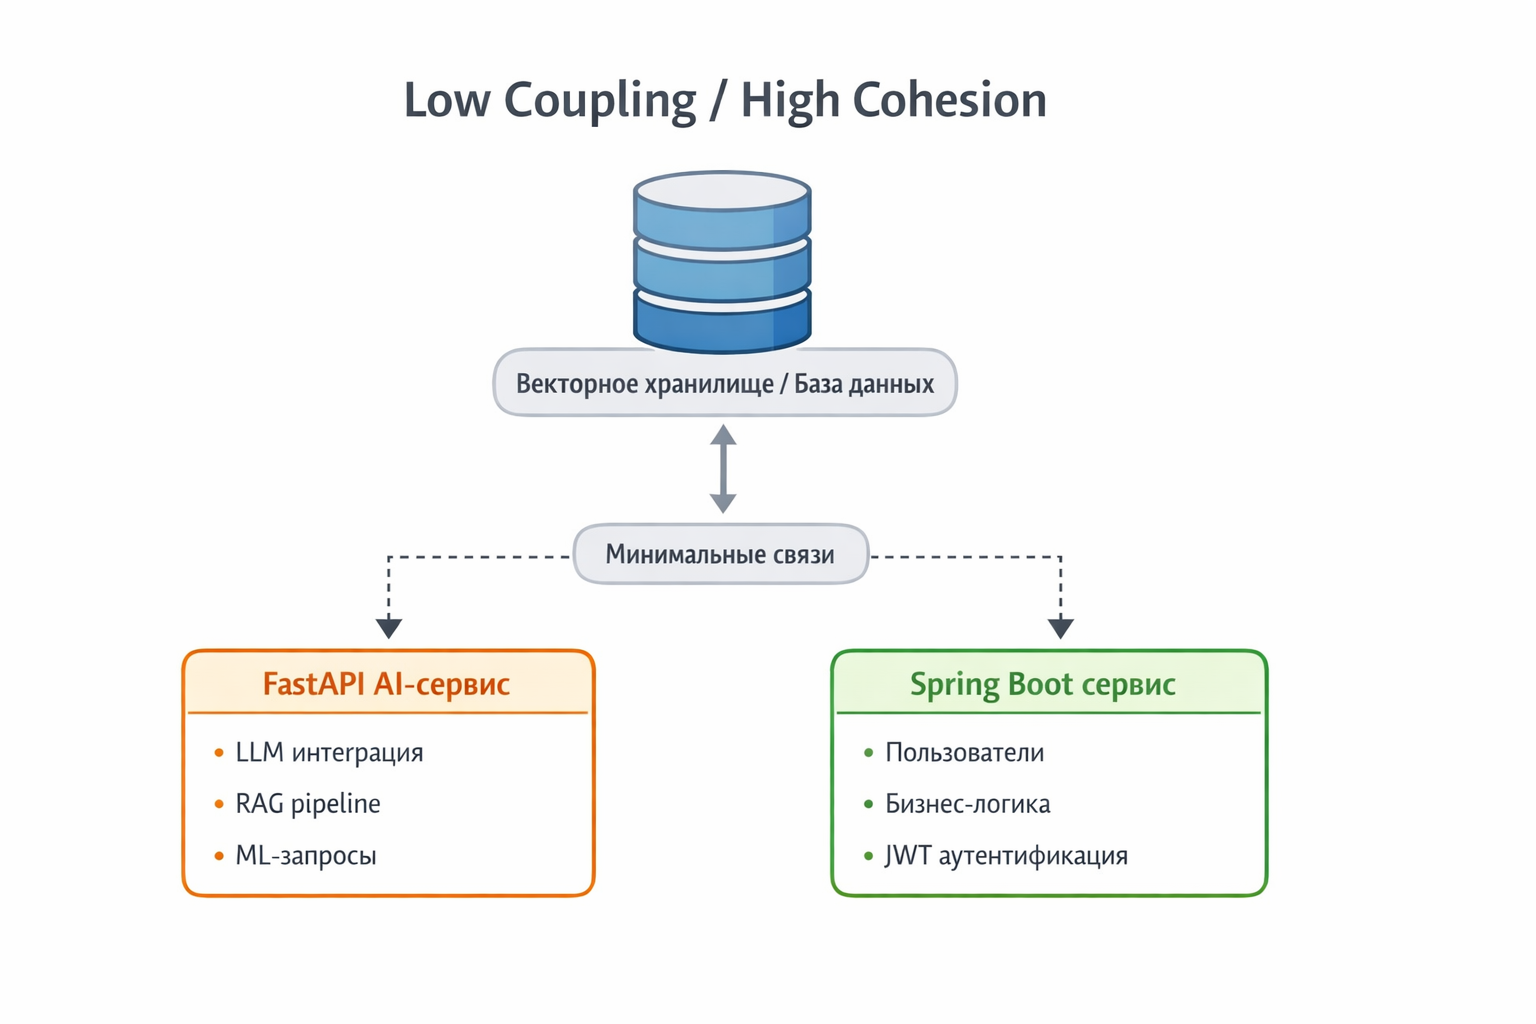
\includegraphics[width=0.85\linewidth]{my_folder/images/image1}
	\caption{Схема схему low coupling / high cohesion}
	\label{fig:1}
\end{figure}


\section{Выбор системы управления базами данных}


\begin{table}[htbp]
	\centering
	\caption{Сравнение СУБД}
	\label{tab:dbms}
	\small
	
\begin{tabular}{|>{\small}p{2.5cm}|>{\small}p{1.5cm}|>{\small}p{3.2cm}|>{\small}p{1.2cm}|>{\small}p{3.4cm}|}
	\hline
		СУБД & Тип & Лицензия & ACID & Комментарий \\
	\hline
		PostgreSQL & SQL & Post\-greSQL License & ++ & Оптимальный выбор \\
	\hline
		MySQL & SQL & GPL & + & Ограничения лицензии \\
	\hline
		MongoDB & NoSQL & SSPL & - & Юридические риски \\
	\hline
		Cassandra & NoSQL & Apache 2.0 & - & Избыточна \\
	\hline
	\end{tabular}

\end{table}


PostgreSQL выбран в качестве основной СУБД по следующим причинам:

\begin{enumerate}
	\item открытая лицензия без ограничений коммерческого использования
	\item строгая транзакционность (ACID)
	\item поддержка JSONB
	\item зрелая интеграция с Spring Data JPA
	\item высокая надежность и масштабируемость
\end{enumerate}

Применение NoSQL-СУБД нецелесообразно, так как проект ориентирован на строгую согласованность пользовательских данных, а также с учетом возможных лицензионных ограничений некоторых NoSQL-платформ.


\section{Выбор векторного хранилища}


\begin{table}[htbp]
	\centering
	\caption{Сравнение векторных хранилищ}
	\label{tab:vector}
	\small
	
\begin{tabular}{|p{2.2cm}|p{2.2cm}|p{2.2cm}|p{2.2cm}|p{2.2cm}|}
	\hline
		Решение & Тип & Стоимость & Контроль данных & Сложность \\
	\hline
		Файловое (PyTorch) & Local & 0 & ++ & + \\
	\hline
		FAISS & Local & 0 & ++ & + \\
	\hline
		Milvus & Server & Средняя & + & ++ \\
	\hline
		Pinecone & Cloud & Высокая & -- & + \\
	\hline
	\end{tabular}

\end{table}


В рамках проекта планируется использование локального файлового векторного хранилища на основе PyTorch-тензоров и вычисления косинусного сходства для реализации семантического поиска в RAG-pipeline.


Преимущества выбранного решения:

\begin{enumerate}
	\item отсутствие дополнительных финансовых затрат
	\item простота развертывания и сопровождения
	\item достаточная производительность для реализации MVP и прототипа системы
\end{enumerate}

\section{Выбор моделей и поставщиков LLM}


Для сценариев работы AI-ассистента придусмотрим интеграцию с внешними языковыми моделями через OpenRouter API. OpenRouter предоставляет единый интерфейс для работы с различными облачными LLM, позволяя использовать любые доступные модели без необходимости интеграции с каждой платформой отдельно. Сервис обеспечивает масштабирование, обновление моделей и управление квотами.


Преимущества:

\begin{enumerate}
	\item Возможность выбирать оптимальную модель для конкретного сценария.
	\item Расширение функционала локальной модели для сложных задач или длинных диалогов.
	\item Быстрое тестирование разных моделей на одном и том же сценарии без сложной настройки.
\end{enumerate}

Недостатки:

\begin{enumerate}
	\item Оплата за использование внешних моделей.
	\item Передача данных третьим сторонам и необходимость соблюдения законодательства о приватности.
\end{enumerate}

\section{Выбор инструмента для расчета времени намаза}


Для реализации функционала расчета времени намаза можно рассмотреть 3 подхода: локальный расчет по формулам, использование сторонней библиотеки или обращение к внешнему API.


1. Локальный расчет по формулам


В данном подходе предполагается самостоятельно рассчитывать времени намаза на основе астрономических формул (положение солнца, географические координаты, временные зоны).


2. Использование внешнего API


В этом подходе предполагается использование сторонних сервисов для получения времени намаза.


3. Использование open source библиотеки


Третий подход заключается в использовании библиотеки Adhan Swift, реализующей расчеты времени намаза непосредственно на устройстве.


\begin{table}[htbp]
	\centering
	\caption{Сравнение методов расчета времени намаза}
	\label{tab:prayer}
	\small
	\begin{tabular}{|p{2.8cm}|p{2.8cm}|p{2.8cm}|p{2.8cm}|}
	\hline
		Критерий & Локальный расчет (формулы) & Библиотека (Adhan Swift) & Внешний API \\
	\hline
		Точность & Зависит от реализации & Высокая, проверенные алгоритмы & Высокая \\
	\hline
		Сложность реализации & Высокая & Низкая & Низкая \\
	\hline
		Поддержка методик расчета & Требуется реализовывать самостоятельно & Встроенная поддержка & Зависит от API \\
	\hline
		Зависимость от интернета & Нет & Нет & Да \\
	\hline
		Поддержка и обновления & Требуется самостоятельно & Обеспечивается библиотекой & Обеспечивается сервисом \\
	\hline
	\end{tabular}
\end{table}


Использование библиотеки Adhan Swift является наиболее рациональным решением, так как он сочетает точность вычислений, простоту интеграции и оффлайн доступ.


\section{Формулирование гипотез}


\textbf{Гипотеза 1}


Применение подхода retrieval-augmented generation, включающего векторный поиск релевантных документов и последующую передачу найденных фрагментов в качестве контекста языковой модели, приводит к повышению точности ответов и снижению частоты галлюцинаций по сравнению с использованием языковой модели без механизма retrieval.


Обоснование:\textbf{ }Использование внешнего контекста позволяет уменьшить зависимость ответа от внутренних представлений языковой модели и обеспечивает опору на проверенные источники, что способствует повышению достоверности и обоснованности генерируемых ответов.


Метод проверки: Проверка гипотезы осуществляется путем сравнения двух режимов функционирования системы: без использования retrieval-механизма и с использованием RAG-подсистемы.


Критерии подтверждения:\textbf{ }Гипотеза считается подтвержденной при выполнении следующих условий:

\begin{enumerate}
	\item увеличение количества корректных ответов
	\item снижение галлюцинаций
\end{enumerate}

\textbf{Гипотеза 2  }


Дообучение модели эмбеддингов на специализированном корпусе (тексты Корана) приводит к повышению качества семантического поиска релевантных документов по сравнению с использованием исходной (базовой) версии модели.


Обоснование: Базовые модели эмбеддингов обучаются на универсальных текстовых корпусах и могут недостаточно точно отражать семантические особенности узкоспециализированной предметной области. Дообучение на специализированном корпусе позволяет адаптировать модель к специфической терминологии и структуре текста.


Метод проверки:\textbf{ }Для каждой рассматриваемой embedding модели проводится сравнение двух состояний: базового (без дообучения) и дообученного на специализированном корпусе. Сравнение осуществляется при фиксированных параметрах генерации и идентичном наборе тестовых запросов. Оценке подлежат релевантность найденных документов и качество итоговых ответов.


Критерии подтверждения: Гипотеза считается подтвержденной при наблюдении:

\begin{enumerate}
	\item увеличение количества корректных ответов
	\item повышения обоснованности ответов
	\item снижения доли нерелевантных источников
\end{enumerate}

\section{Проектирование общей схемы взаимодействия компонентов}


Спроектируем общую схему взаимодействия компонентов системы. Система будет состоять из трех основных частей: iOS-приложение, которое является точкой входа для пользователя, Spring Boot backend, отвечающий за аутентификацию, бизнес-логику и работу с базой данных и FastAPI LLM-сервис, изолированный в отдельный микросервис в соответствии с принципом low coupling, рассмотренным в разделе 2.4. Запросы к AI-ассистенту будут проходить через Spring Boot и проксироваться в LLM-сервис. Каждый из компонентов более подробно будет рассмотрен в пунктах ниже.


\begin{figure}[H]
	\centering
	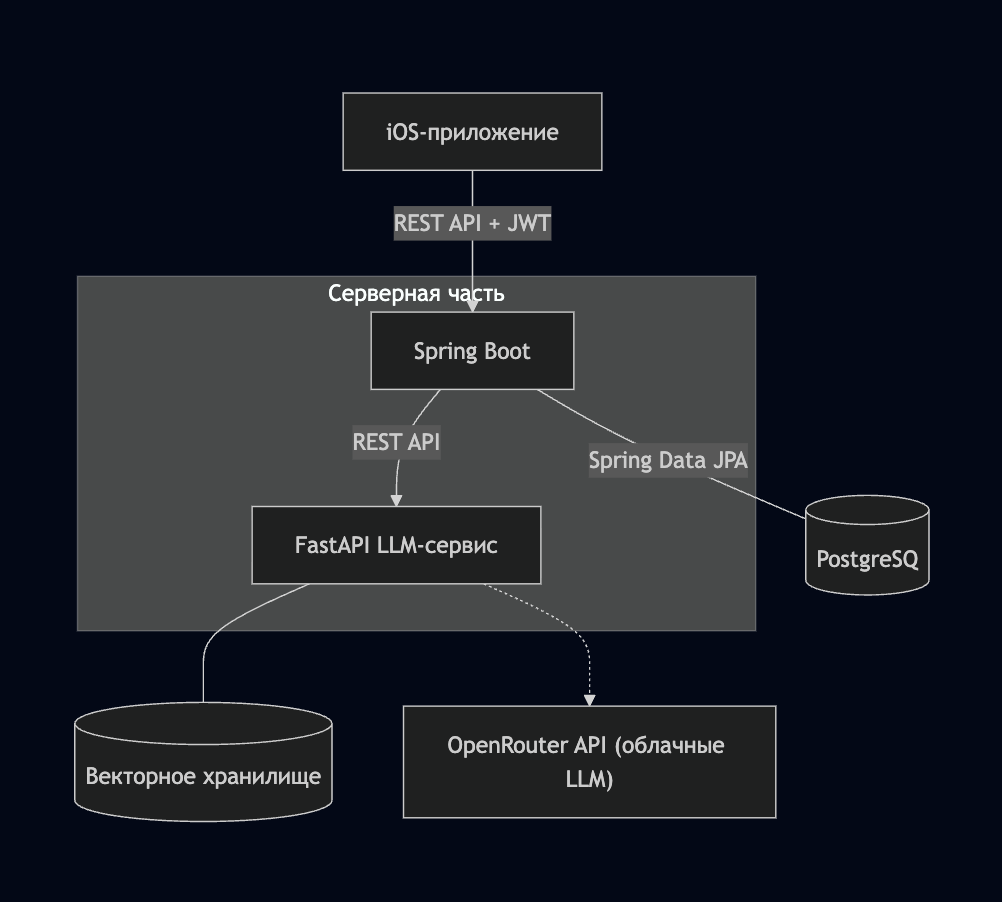
\includegraphics[width=0.85\linewidth]{my_folder/images/image2}
	\caption{Общая схема взаимодействия компонентов системы}
	\label{fig:2}
\end{figure}


\section{Use Case диаграммы}


Диаграмма вариантов использования (Use Case Diagram) описывает функциональные возможности системы с точки зрения пользователя, определяя доступные в приложении действия без рассмотрения вопросов внутренней реализации. Она представляет собой первый этап проектирования, позволяющий зафиксировать все пользовательские сценарии до перехода к разработке диаграмм классов и алгоритмов.


В системе выделены три актора: гость, авторизованный пользователь и система. Гость - это пользователь, который запускает приложение без авторизации. Такой режим позволяет использовать базовые функции приложения без создания учетной записи, что снижает барьер входа для новых пользователей и позволяет ознакомиться с возможностями приложения. В режиме гостя доступен просмотр религиозного контента, а также информация о времени намаза.


Авторизованный пользователь обладает расширенными возможностями. Он наследует все варианты использования гостя и дополнительно получает доступ к функционалу сканера продуктов, AI-ассистента и расширенным настройкам приложения. Использование авторизации обусловлено необходимостью хранения персональных настроек пользователя, а также управлением доступом к расширенным функциям системы.


\begin{figure}[H]
	\centering
	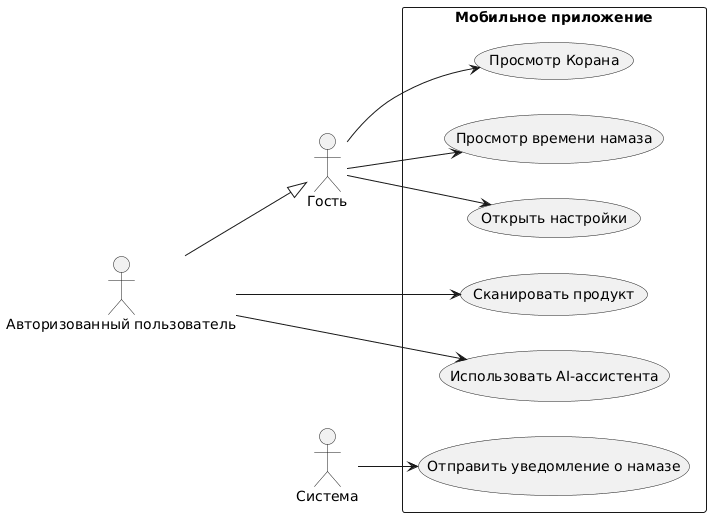
\includegraphics[width=0.85\linewidth]{my_folder/images/image3}
	\caption{Общая диаграмма вариантов использования системы}
	\label{fig:3}
\end{figure}


Все варианты использования объединены в шесть функциональных блоков:

\begin{enumerate}
	\item Модуль аутентификации отвечает за идентификацию пользователя и предоставление доступа к персонализированным функциям приложения. Незарегистрированный пользователь может зарегистрироваться, войти в систему или продолжить работу в режиме гостя. После успешной аутентификации пользователь получает доступ к расширенным возможностям приложения.
\end{enumerate}

\begin{figure}[H]
	\centering
	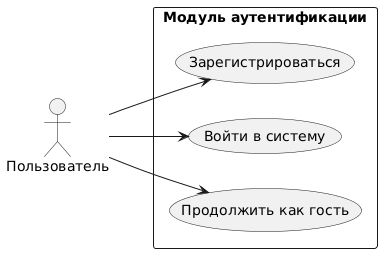
\includegraphics[width=0.6375\linewidth]{my_folder/images/image4}
	\caption{Use Case-диаграмма модуля аутентификации}
	\label{fig:4}
\end{figure}

\begin{enumerate}
	\setcounter{enumi}{1}
	\item Модуль сканера продуктов предназначен для анализа состава пищевых продуктов и определения их соответствия требованиям халяль. Основной пользовательский сценарий "Проверить состав продукта" доступен только авторизованным пользователям и может быть запущен через камеру устройства или из галереи изображений. Распознавание текста и классификация ингредиентов являются обязательными этапами обработки данных и включены в основной сценарий через отношение <<include>>. Ручной ввод состава реализован как альтернативный путь выполнения и обозначен связью <<extend>>.
\end{enumerate}

\begin{figure}[H]
	\centering
	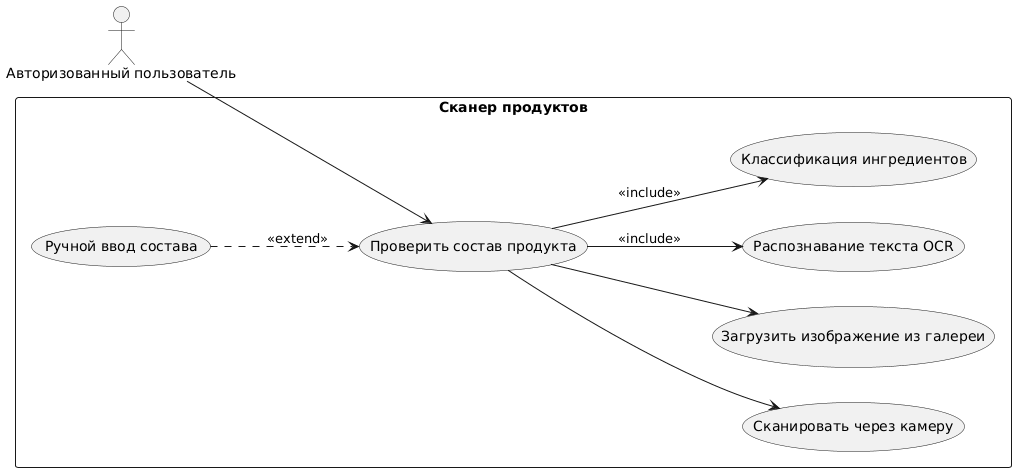
\includegraphics[width=0.85\linewidth]{my_folder/images/image5}
	\caption{Use Case-диаграмма модуля "Сканер продуктов"}
	\label{fig:5}
\end{figure}

\begin{enumerate}
	\setcounter{enumi}{2}
	\item Модуль AI-ассистента предоставляет пользователю возможность задавать вопросы, связанные с халяльностью продуктов и ингредиентов. При каждом обращении к ассистенту автоматически формируется контекст для генерации ответа на основе механизма retrieval-augmented generation (RAG), что обозначено отношением <<include>>. Использование удаленной языковой модели через сервис OpenRouter реализовано как расширение основного сценария (<<extend>>) и активируется только в случае, если пользователь указал API-ключ в настройках приложения.
\end{enumerate}

\begin{figure}[H]
	\centering
	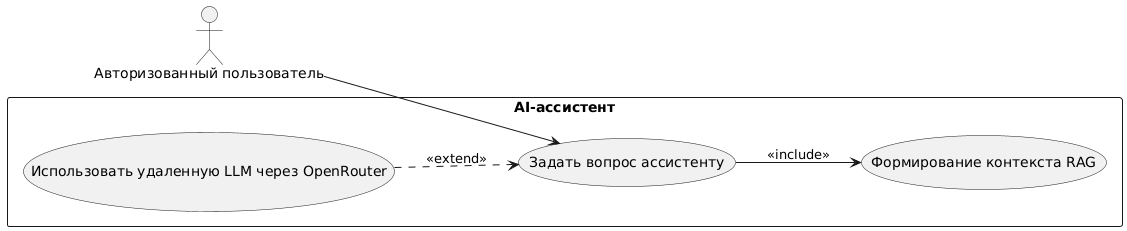
\includegraphics[width=0.85\linewidth]{my_folder/images/image6}
	\caption{Use Case-диаграмма модуля AI-ассистента}
	\label{fig:6}
\end{figure}

\begin{enumerate}
	\setcounter{enumi}{3}
	\item Модуль Коран предоставляет пользователю возможность просматривать список сур и читать выбранные суры и аяты. Данный функционал доступен как гостю, так и авторизованному пользователю.
	\item Модуль времени намаза отображает расписание пяти обязательных намазов на текущий день, рассчитанное на основе геолокации пользователя. Система автоматически отправляет уведомления в назначенное время. Пользователь может дополнительно настроить уведомления для каждого намаза, что реализовано как расширение основного сценария через связь <<extend>>.
	\item Модуль настроек предназначен для управления параметрами приложения. В режиме гостя пользователю доступна возможность перейти к авторизации. После входа в систему открываются дополнительные функции: управление API-ключом для удаленных моделей, выбор используемой языковой модели (LLM), настройка параметра генерации max\_tokens, а также выход из аккаунта.
\end{enumerate}

\begin{figure}[H]
	\centering
	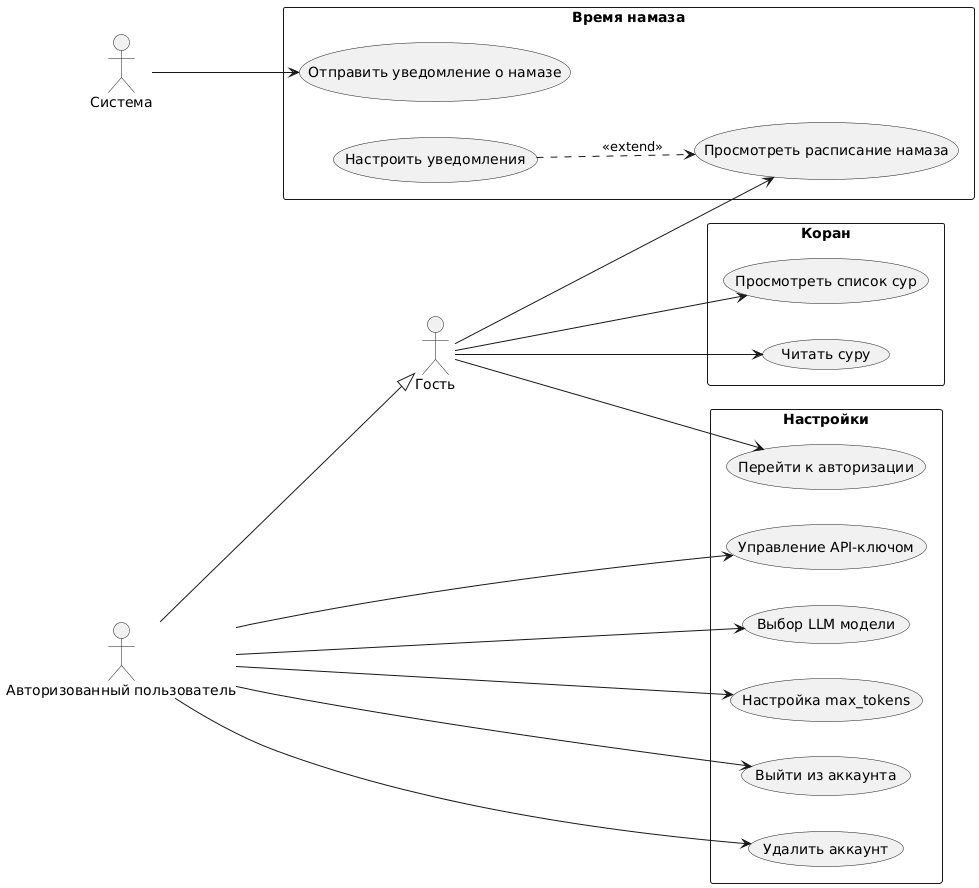
\includegraphics[width=0.85\linewidth]{my_folder/images/image7}
	\caption{Use Case-диаграмма модулей "Коран", "Время намаза" и "Настройки"}
	\label{fig:7}
\end{figure}


\section{Схема базы данных}


В разделе 1.5 была выбрала PostgreSQL качестве СУБД. Планируется создание двух таблиц: для хранения пользовательских аккаунтов и текстов Корана (см. рисунок~\ref{fig:2}).


\begin{figure}[H]
	\centering
	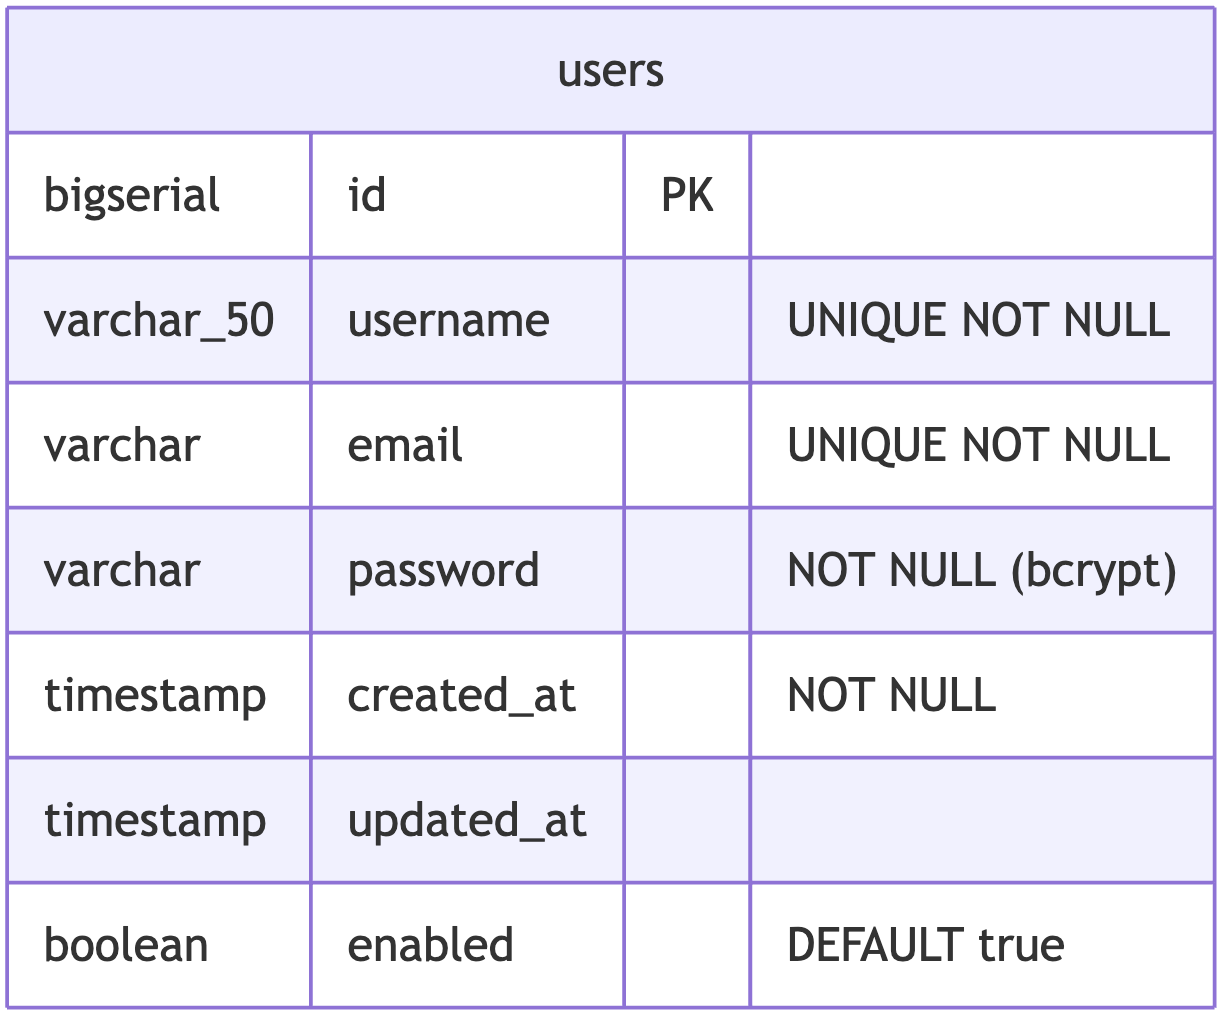
\includegraphics[width=0.6375\linewidth]{my_folder/images/image8}
	\caption{Таблица users}
	\label{fig:8}
\end{figure}


\begin{figure}[H]
	\centering
	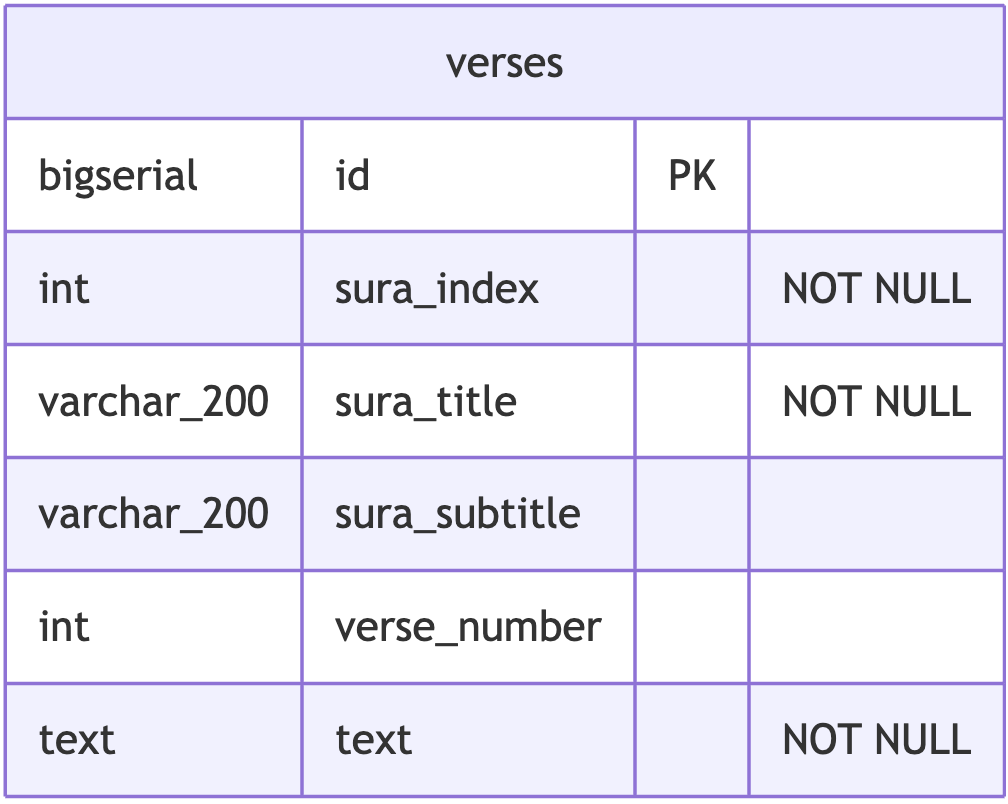
\includegraphics[width=0.6375\linewidth]{my_folder/images/image9}
	\caption{Таблица verses}
	\label{fig:9}
\end{figure}


Для LLM-сервиса планируется использовать файловое векторное хранилище - бинарный файл формата PyTorch. Он будет содержать два объекта: список документов (фрагменты аятов с метаданными) и матрицу эмбеддингов размерностью N на D, где N - это количество проиндексированных фрагментов, а D - размерность векторного представления выбранной модели эмбеддингов. Значение D определяется моделью: например, для paraphrase-multilingual-MiniLM-L12-v2 оно составляет 384, для более тяжелых моделей 768 или 1024. Окончательный выбор модели планируется произвести по результатам экспериментов в главе о разработке. Поиск векторному хранилищу будет выполняться через косинусное сходство, поэтому он намеренно выносится за пределы PostgreSQL - обновление индекса не должно затрагивать основную базу данных.


\begin{figure}[H]
	\centering
	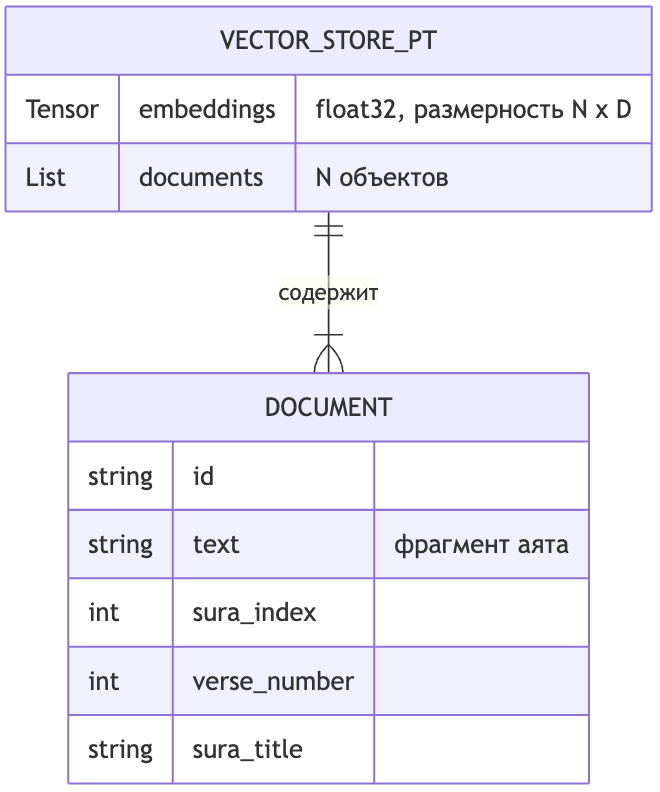
\includegraphics[width=0.6375\linewidth]{my_folder/images/image10}
	\caption{Структура векторного хранилища}
	\label{fig:10}
\end{figure}


\section{Алгоритмы обработки данных}


Рассмотрим 3 основных алгоритма, каждый из которых соответствует отдельному функциональному модулю приложения:

\begin{enumerate}
	\item Алгоритм обработки чат-запроса с использованием RAG. Он описывает процесс от получения пользовательского сообщения до формирования ответа.
	\item Алгоритм анализа состава продукта. Он описывает процесс от выбора источника изображения до классификации каждого ингредиента по категориям "халяль", "харам" и "сомнительный" с формированием итогового вердикта о продукте.
	\item Алгоритм расчета времени намаза. Он рассчитывает время намаза на основе астрономических формул, координат пользователя и выбранного метода расчета.
\end{enumerate}

\subsection{Алгоритм обработки чат-запроса с использованием RAG}


Алгоритм обработки чат-запроса выполняется на стороне LLM-сервиса, реализованного на языке Python с использованием веб-фреймворка FastAPI. Запросы поступают от backend-сервиса, который проксирует их в соответствии с принципом слабой связности (low coupling), рассмотренным в разделе 2.4. На вход алгоритм принимает следующие параметры: история диалога в формате последовательности сообщений с указанием ролей участников, максимальное количество токенов в генерируемом ответе,  идентификатор языковой модели и API-ключ пользователя для доступа к OpenRouter.


Сам алгоритм состоит из нескольких этапов.


Первый этап - это предобработка и извлечение поискового запроса. Система последовательно проходит по всем сообщениям в обратном хронологическом порядке и выделяет первое сообщение, чей отправитель имеет роль пользователя. Выделенное сообщение представляет собой основной поисковый запрос. История диалога сохраняется в полном объеме для контекстуализации ответа от LLM.


На втором этапе семантический поиск в базе знаний с помощью RAG. Извлеченный поисковый запрос векторизируется. Данное преобразование выполняется таким образом, чтобы семантически связанные тексты получали близкие векторные представления. Полученный вектор запроса сравнивается со всеми векторными представлениями документов, хранящихся в базе знаний (аятов Корана), посредством вычисления функции косинусного сходства.


\begin{figure}[H]
	\centering
	
\includegraphics[width=0.85\linewidth]{my_folder/images/image11}
	\caption{Формула вычисления косинусного сходства}
	\label{fig:11}
\end{figure}


На основе вычислений выбираются 3 наиболее релевантных результата. Для каждого выбранного документа сохраняются данные: номер суры, номер аята, текст аята, значение функции сходства.


Далее происходит формирование входных данных для языковой модели (см. рисунок~\ref{fig:12}). Выбранные источники объединяются в текстовый блок, где каждый источник содержит: номер суры, номер аята, полный текст аята. К сформированному блоку добавляется системный промпт, содержащий инструкции для языковой модели:

\begin{enumerate}
	\item базировать ответы исключительно на предоставленных источниках.
	\item приводить в ответе конкретные ссылки на номера сур и аятов.
	\item воздерживаться от ответа при отсутствии релевантной информации в контексте.
\end{enumerate}

Подготовленная последовательность сообщений отправляется в удаленную языковую модель через API OpenRouter. Когда языковая модель возвращает результат он отображается у пользователя в чате и добавляется в историю сообщений для обогащения контекста.


\begin{figure}[H]
	\centering
	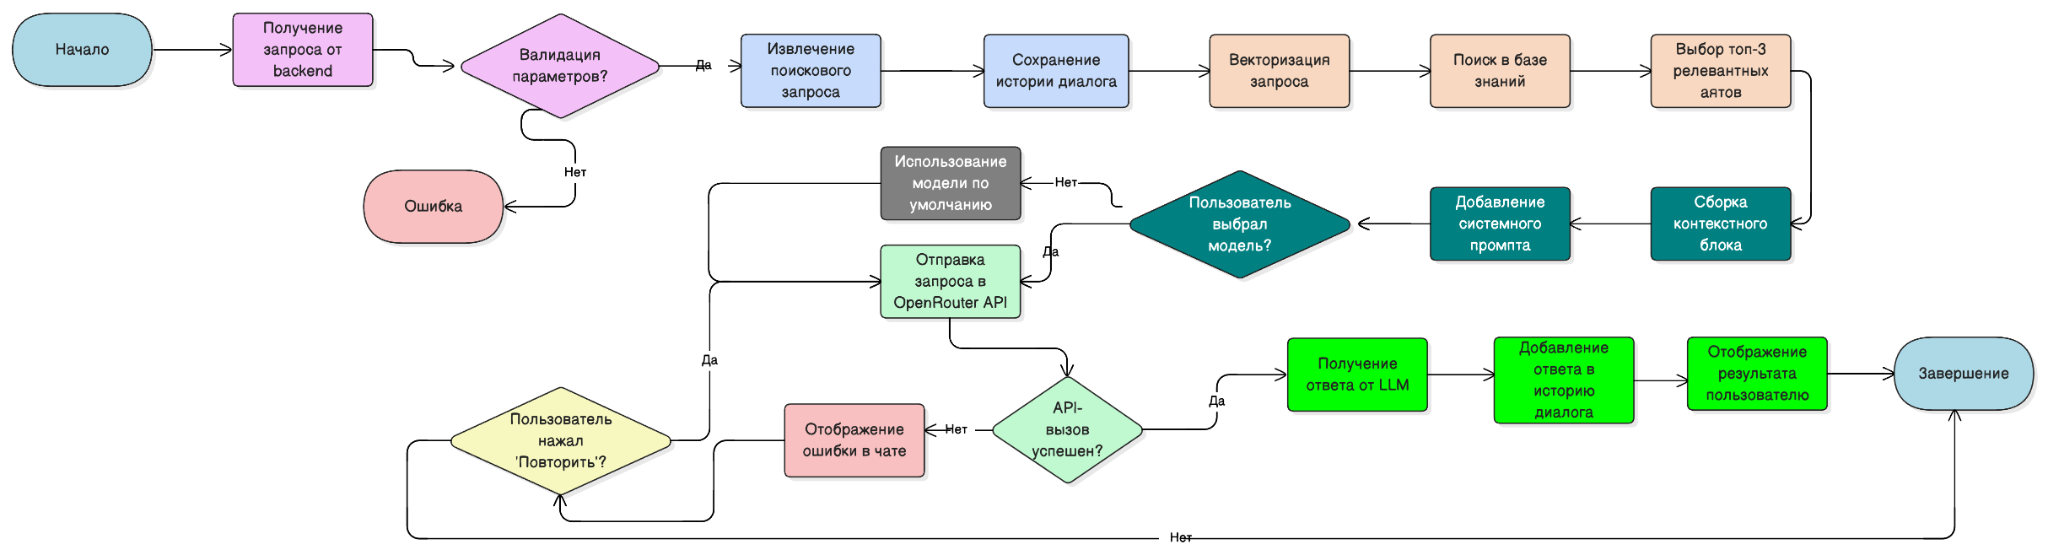
\includegraphics[width=0.85\linewidth]{my_folder/images/image12}
	\caption{Блок-схема алгоритма анализа состава продукта}
	\label{fig:12}
\end{figure}


\subsection{Алгоритм анализа состава продукта}


Алгоритм анализа состава планируется реализовать полностью на стороне клиента. База ингредиентов будет храниться локально в приложения в CSV-файла и загружаться в память при первом запуске.


Алгоритм предполагает два возможных пути получения входных данных: фотографирование упаковки (или выбор из галереи) и ручной ввод текста состава. В первом случае перед анализом выполняется этап распознавания текста - изображение обрабатывается OCR-движком, результаты с нескольких фотографий объединяются в одну строку. При ручном вводе текст поступает на анализ напрямую.


Поскольку качество распознавания зависит от освещения, угла съемки и шрифта на упаковке, планируется предусмотреть информационный дисклеймер, который будет отображаться пользователю вместе с результатами анализа. Он будет содержать предупреждение о том, что результат основан на автоматически распознанном тексте, и рекомендацию самостоятельно убедиться в корректности считанного состава перед принятием решения о покупке или употреблении.


Анализ текста планируется разбить на два независимых шага, которые выполняются последовательно.


Первым шагом выполняется поиск по E-кодам. Из текста извлекаются все токены вида "E" + цифры (например, E471, E120). Каждый найденный код сверяется с базой ингредиентов по точному совпадению. Найденные ингредиенты исключаются из дальнейшего поиска во втором шаге.


Второй шаг - это поиск по названиям. Для каждого ингредиента из базы, не найденного на первом шаге, выполняется нечеткое сопоставление с текстом по русскому и английскому названиям. Каждому совпадению присваивается оценка (score) в диапазоне от 0 до 1. Точное совпадение названия ингредиента с текстом по границам слов дает score = 1.0. Для частичных совпадений вычисляется matchRatio - это доля значимых слов названия (длиной от 4 символов), найденных в тексте: например, если название содержит 3 значимых слова и 2 из них обнаружены в тексте, matchRatio = 0.67. Итоговый score для частичных совпадений вычисляется как matchRatio * 0.85. Коэффициент 0.85 намеренно снижает оценку относительно точного совпадения, чтобы при финальной фильтрации точные совпадения всегда имели приоритет над частичными. Кандидаты с оценкой ниже 0.7 отбрасываются. Затем из оставшихся кандидатов удаляются дублирующие подмножества. Например, если в тексте найдено и "молоко", и "сухое молоко", остается более специфичное совпадение.


После объединения результатов обоих шагов выставляется итоговый статус продукта по приоритетной схеме: наличие хотя бы одного харам-ингредиента делает продукт харамом вне зависимости от остальных, при отсутствии харам, но наличии сомнительных - статус "сомнительный", если все найденные ингредиенты халяль - статус "халяль", если не удалось распознать, то статус "неизвестно".


\begin{figure}[H]
	\centering
	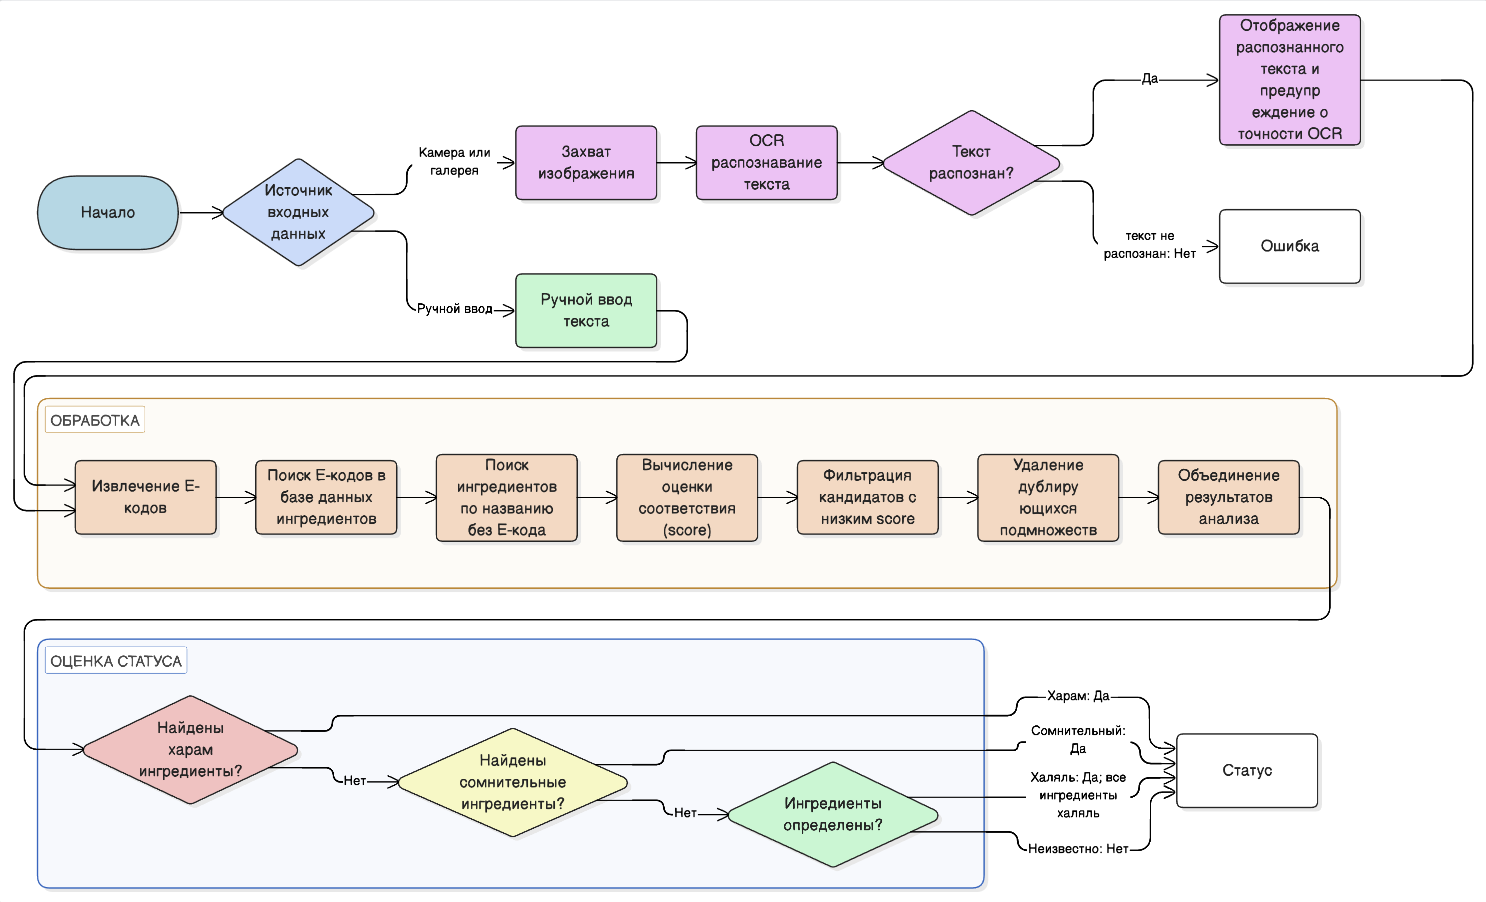
\includegraphics[width=0.85\linewidth]{my_folder/images/image13}
	\caption{Блок-схема алгоритма анализа состава продукта}
	\label{fig:13}
\end{figure}


\subsection{Алгоритм расчета времени намаза}


Алгоритм расчета времени намаза реализуется полностью на стороне клиента (iOS) без обращения к серверу. В качестве вычислительного ядра используется библиотека Adhan Swift. Такой подход обеспечивает возможность работы в офлайн-режиме, снижает задержки при получении результатов и исключает зависимость от внешних сетевых сервисов.


В основе алгоритма лежат три группы входных данных: географические координаты пользователя (широта и долгота), дата (год, месяц, день), а также параметры расчета, задаваемые пользователем.


Параметры расчета включают несколько важных аспектов. Во-первых, это метод расчета времени намаза, представляющий собой набор правил и астрономических параметров, используемых в различных регионах мира. Разные исламские организации (например, в Саудовской Аравии, Турции, Европе) используют различные углы положения Солнца для определения начала некоторых молитв, что приводит к небольшим различиям во времени. Выбор метода позволяет адаптировать расчет под региональные стандарты.


Во-вторых, учитывается мазхаб - правовая школа в исламе, которая влияет на определение времени наступления молитвы Аср. В частности, различие заключается в длине тени объекта: в шафиитской традиции Аср начинается, когда длина тени равна длине самого объекта, а в ханафитской - когда тень в два раза длиннее объекта. Это приводит к различию во времени начала данной молитвы.


Дополнительно могут задаваться пользовательские параметры для молитв Фаджр и Иша, которые определяются по углу положения Солнца относительно горизонта. Фаджр - это утренняя молитва, начинающаяся до восхода Солнца, а Иша --- ночная молитва, наступающая после наступления темноты. Время этих молитв зависит от того, на сколько градусов Солнце опускается ниже горизонта (например, 18$^{\circ}$, 15$^{\circ}$ и т.д.). Пользователь может задать эти значения вручную для более точной настройки расчета.


Поскольку точность вычислений напрямую зависит от корректности геолокации и системного времени устройства, в пользовательском интерфейсе предусмотрены состояния, информирующие о невозможности выполнения расчета. В частности, при отсутствии доступа к геолокации или невозможности определить координаты пользователю отображается соответствующее сообщение, а расчет не производится.


Алгоритм включает несколько последовательных этапов. На первом этапе выполняется получение и валидация местоположения пользователя. Приложение запрашивает разрешение на доступ к геолокации, после согласия пользователя мы получаем текущие координаты с точностью, достаточной для расчета времени намаза. При отсутствии координат дальнейшие вычисления не выполняются.


Далее формируются параметры расчета. В зависимости от выбранного пользователем метода задаются соответствующие параметры. Если пользователь задал собственные значения углов для Фаджра и Иши, они имеют приоритет и подменяют стандартные параметры метода.


На следующем этапе осуществляется непосредственный расчет времени молитв. На основе календарной даты формируются необходимые компоненты, после чего библиотеке передаются координаты, дата и параметры. В результате вычисляются временные метки для шести событий дня: Фаджр, Шурук, Зухр, Аср, Магриб и Иша. В случае невозможности выполнения вычислений результат считается недоступным.


Заключительный этап включает постобработку полученных данных и определение ближайшей молитвы. Результаты преобразуются во внутреннюю модель приложения, после чего определяется ближайшее предстоящее событие. Для этого выбирается первое время молитвы, превышающее текущий момент. Если все молитвы текущего дня уже прошли, система фиксирует соответствующее состояние.


\begin{figure}[H]
	\centering
	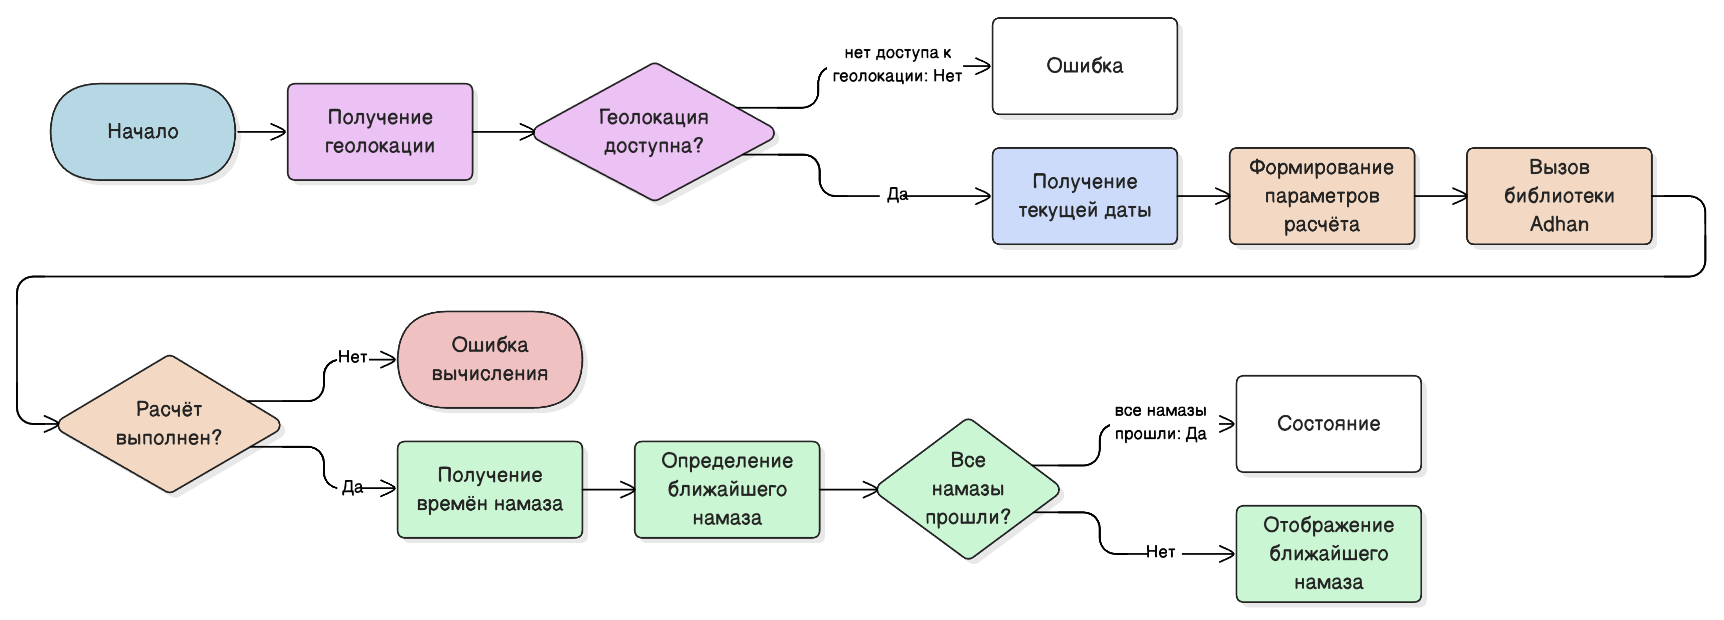
\includegraphics[width=0.85\linewidth]{my_folder/images/image14}
	\caption{Блок-схема алгоритма расчета времени намаза}
	\label{fig:14}
\end{figure}


\section{Проектирование REST API}


Для обеспечения взаимодействия между компонентами системы используется REST API. Данный интерфейс определяет контракты обмена данными между iOS-приложением, backend-сервером и LLM-сервисом.


\begin{table}[htbp]
	\centering
	\caption{REST API эндпоинты}
	\label{tab:api}
	\small
	
\begin{tabular}{|>{\small}p{1.7cm}|>{\small}p{1.3cm}|>{\small}p{3.8cm}|>{\small}p{3.5cm}|>{\small}p{3.5cm}|}
	\hline
		Сервис & Метод & Endpoint & Request & Response \\
	\hline
		Auth & POST & /api/auth/register & username, email, password & JWT токен + данные пользователя \\
	\hline
		Auth & POST & /api/auth/login & username/email, password & JWT токен + данные пользователя \\
	\hline
		Auth & POST & /api/auth/refresh & refresh token & новый JWT токен \\
	\hline
		Quran & GET & /api/verse-of-the-day & - & аят (сура, текст, номер) \\
	\hline
		Chat & POST & /api/chat & messages[], model, api\_key & ответ модели \\
	\hline
		Chat & GET & /api/models & - & список моделей \\
	\hline
		LLM Service & GET & /llm/health & - & status, готовность RAG/LLM \\
	\hline
		LLM Service & POST & /llm/chat & messages[], параметры & ответ модели \\
	\hline
	\end{tabular}

\end{table}


Рассмотрим каждый endpoint более подробно.

\begin{enumerate}
	\item /api/auth/register (POST)

	Endpoint предназначен для регистрации нового пользователя в системе. В теле запроса передаются имя пользователя, адрес электронной почты и пароль. В случае успешной регистрации сервер создает учетную запись, формирует JWT-токен доступа и возвращает его вместе с основными данными пользователя.

	\item /api/auth/login (POST)

	Endpoint используется для аутентификации ранее зарегистрированного пользователя. В запросе передаются учетные данные пользователя: имя пользователя или адрес электронной почты, а также пароль. В ответ сервер возвращает JWT-токен доступа и сведения о пользователе.

	\item /api/auth/refresh (POST)

	Endpoint предназначен для обновления access token без повторного ввода логина и пароля. В теле запроса передается refresh token, на основе которого сервер формирует новый JWT-токен доступа. Использование данного endpoint позволяет поддерживать пользовательскую сессию и повышает удобство использования приложения.

	\item /api/verse-of-the-day (GET)

	Endpoint используется для получения случайного аята дня. Запрос не требует передачи параметров. В ответ сервер возвращает информацию об аяте, включая номер суры, номер аята и текст.

	\item /api/chat (POST)

	Endpoint является основным входом для работы чат со стороны клиента. В теле запроса передается история сообщений, а также дополнительные параметры генерации, такие как выбранная модель и API-ключ пользователя для удаленной LLM. Backend-сервис принимает этот запрос, выполняет необходимую обработку и проксирует его в LLM-service. В ответ клиент получает сформированный текст ответа модели. Таким образом, данный endpoint выступает связующим звеном между iOS-приложением и LLM-service.

	\item /api/models (GET)

	Endpoint предназначен для получения списка доступных языковых моделей, которые могут быть использованы в системе. Запрос не требует передачи параметров. В ответ возвращается список моделей, доступных для выбора пользователем в настройках приложения.

	\item /llm/health (GET)

	Endpoint используется для проверки состояния LLM-service. В ответ возвращается информация о доступности сервиса, а также о готовности его ключевых компонентов, в частности RAG-подсистемы и модуля взаимодействия с языковой моделью.

	\item /llm/chat (POST)

	Endpoint является основным для обработки чат-запросов в LLM-service. В теле запроса передается история сообщений пользователя, а также параметры генерации ответа, включая API-ключ, максимальное количество токенов и название удаленной модели. После получения запроса сервис выполняет извлечение поискового запроса, поиск релевантных фрагментов Корана с использованием RAG и обращение к внешней языковой модели через OpenRouter. В ответ возвращается готовый текст.
\end{enumerate}


\section{Архитектура iOS-приложения}


\subsection{Общее описание архитектурного подхода}


iOS-приложение будет разработано с модульной многоуровневой архитектурой. Реализация будет выполнена на языке Swift с применением декларативного фреймворка SwiftUI


Предварительно разделим код на следующие слои (см. рисунок~\ref{fig:16}):

\begin{enumerate}
	\item Слой представления (Presentation Layer) - отвечает за отображение пользовательского интерфейса и обработку действий пользователя.
	\item Слой координации навигации (Navigation Coordination Layer) - управляет переходами между экранами и навигационными сценариями приложения.
	\item Слой бизнес-логики (Business Logic Layer) - содержит сервисы, реализующие прикладную логику и координирующие обработку данных.
	\item Слой данных (Data Layer) - отвечает за взаимодействие с backend-сервисами, локальными хранилищами и другими источниками данных.
\end{enumerate}

\subsection{Управление навигацией через паттерн Coordinator}


Для управления навигацией будет использован паттерн Coordinator при котором  логика переходов выносится из представлений и инкапсулируется в отдельном объекте - координаторе.


Глобальный координатор будет хранить стек активных экранов и управлять переходами между ними. Для каждой основной области приложения (чат, главный экран, настройки) будут созданы специализированные координаторы, которые управляют навигацией внутри этой области.


Данный подход позволяет легко добавлять новые сценарии навигации и делать контроллеры представления легковесными и сосредоточенными только на представлении данных и реагировании на ввод пользователя. Поскольку контроллеры представлений не будут обрабатывают навигацию, становится проще их логику изолированно.


\subsection{Внедрение зависимостей}


Все сервисы и компоненты приложения создаются и управляются с использованием контейнера зависимостей (DependencyContainer). Контейнер зависимостей - это инструмент, позволяющий управлять, регистрировать и разрешать зависимости в приложении. Это не только упрощает процесс разработки и тестирования, но и повышает модульность и повторное использование кода.


Для создания экранов применяется фабричный подход (ScreenFactory). При необходимости отображения нового экрана приложение обращается к фабрике, которая формирует экземпляр экрана и внедряет в него все требуемые зависимости.


Основным преимуществам данного подхода является: централизованное управление зависимостями, возможность замены реальных сервисов на тестовые реализации(моки и стабы), снижение связности между компонентами системы.


\subsection{Сервисы}


Бизнес-логика будет реализована с помощью сервисов. Каждый сервис отвечает за конкретную область: управление чатом, аутентификация, работа с Кораном, геолокация, расписание молитв и т. д


Сервисы будут определены через протоколы (интерфейсы), что позволит легко менять их реализацию без изменения существующего кода. Реактивность будет достигнута через макрос @Observable, когда состояние сервиса меняется, все связанные экраны обновляются автоматически.


\subsection{Экраны и их состояние}


Для организации кода каждого экрана используется архитектурный паттерн MVVM (Model-View-ViewModel), предполагающий разделение на три компонента.


View (представление) - это пользовательский интерфейс, реализованный с использованием SwiftUI. View отвечает исключительно за отображение данных и передачу пользовательских действий во ViewModel. Представление не содержит бизнес-логики и не определяет источник данных.


ViewModel (модель представления) - компонент, связанный с View и отвечающий за управление состоянием экрана. ViewModel выполняет следующие функции: управление состоянием, обработку пользовательских действий, а также преобразование данных, получаемых из сервисов, в формат, удобный для отображения.


Model (модель) - слой, представленный сервисами, содержащими бизнес-логику и данные приложения. Model не зависит от View и ViewModel и предоставляет методы для работы с состоянием.


\begin{figure}[H]
	\centering
	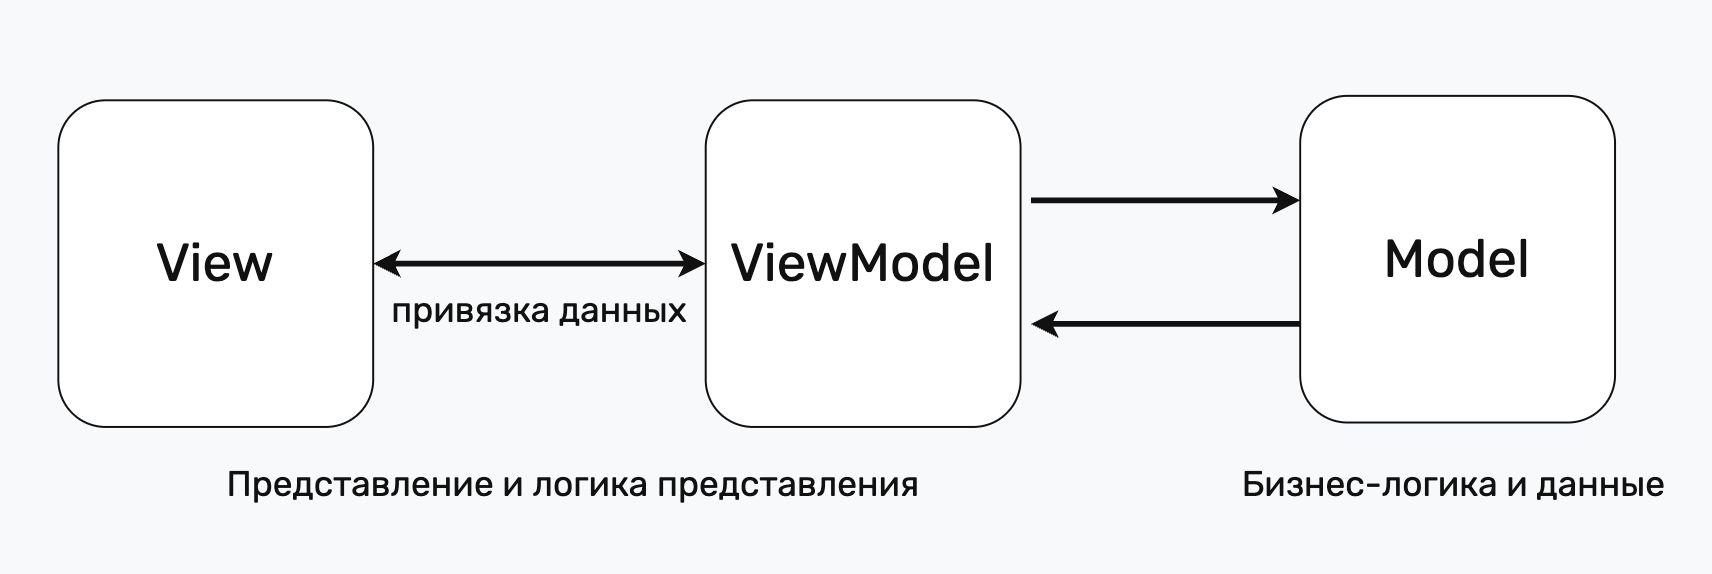
\includegraphics[width=0.85\linewidth]{my_folder/images/image15}
	\caption{MVVM}
	\label{fig:15}
\end{figure}


\subsection{Взаимодействие с backend}


Взаимодействие приложения с backend-сервисом осуществляется посредством HTTP-запросов. Все сетевые операции выполняются асинхронно, что позволяет избежать блокировки пользовательского интерфейса и обеспечить корректную работу приложения.


Для управления сетевыми запросами выделяется NetworkLayer. Он представляет собой абстракцию над механизмами HTTP-коммуникации. Данный слой инкапсулирует следующие функции: формирование запросов (URL, заголовки, параметры), отправка запросов на backend-сервис, обработка ответов и ошибок, преобразование полученных данных во внутренний формат приложения. Это позволяет изолировать детали реализации сетевого взаимодействия от бизнес-логики. В результате сервисы не зависят от конкретного способа коммуникации с backend-сервисом. Это обеспечивает гибкость архитектуры: при необходимости изменения протокола взаимодействия (например, перехода на WebSocket) изменения затрагивают только NetworkLayer, не влияя на остальные компоненты системы.


\begin{figure}[H]
	\centering
	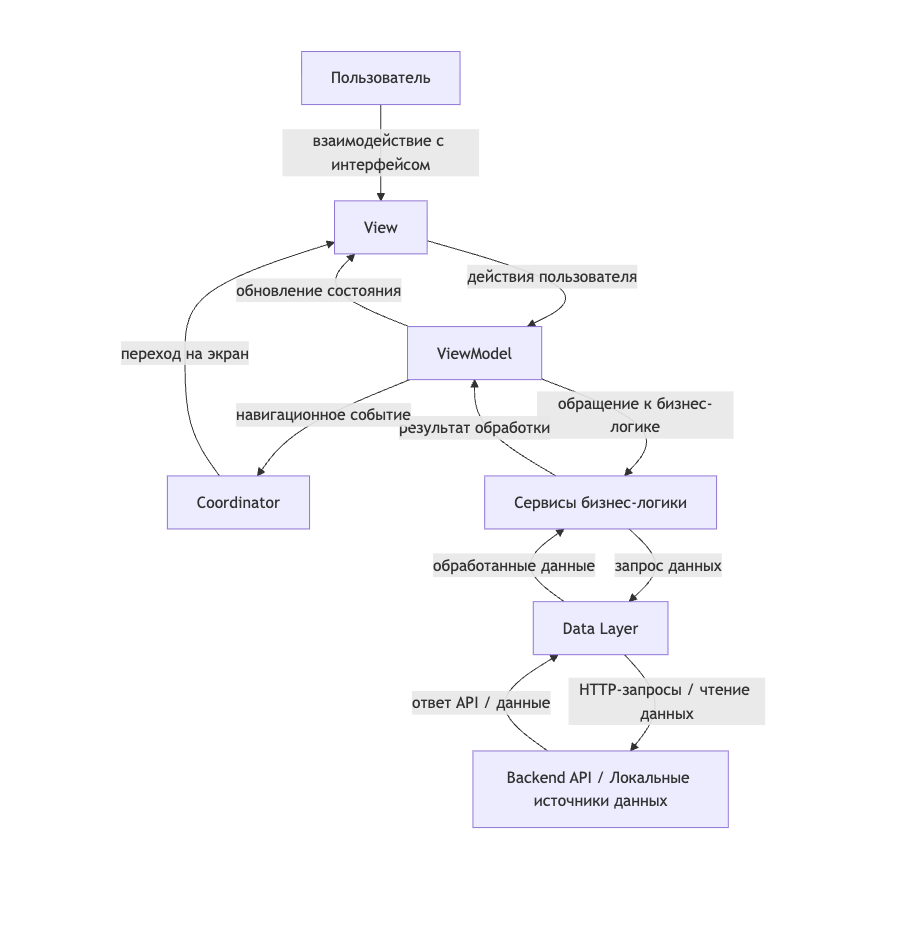
\includegraphics[width=0.85\linewidth]{my_folder/images/image16}
	\caption{Архитектура iOS-приложения}
	\label{fig:16}
\end{figure}


\section{Архитектура Backend}


Backend-сервер будет разработан на Java с использованием фреймворка Spring Boot. Он отвечает за управление пользователями, хранение данных и предоставляет REST API, с которым взаимодействует iOS-приложение.


Архитектура backend-сервера построена по трехслойной модели: слой API, слой бизнес-логики и слой данных.


\subsection{Трехслойная архитектура}


Слой API определяет HTTP-эндпоинты, к которым обращается iOS-приложение. Каждый эндпоинт реализует конкретную функциональность, например: аутентификацию, получение профиля пользователя, работу с чатом или поиск ингредиентов. Данный слой не содержит бизнес-логики. Его основная задача - принять запрос, передать его в слой бизнес-логики и вернуть сформированный ответ клиенту.


В слой бизнес-логики реализуется основная логика приложения. Здесь выполняется валидация данных, проверка прав доступа и применение бизнес-правил. Этот слой не зависит от способа взаимодействия с клиентом и работает с абстрактными данными и моделями.


Слой данных отвечает за взаимодействие с базой данных PostgreSQL. Для работы с данными используется Spring Data JPA, которая позволяет оперировать объектами вместо написания SQL-запросов вручную. ORM автоматически преобразует операции над объектами в соответствующие SQL-запросы.


\subsection{Аутентификация через JWT}


Для аутентификации пользователей используется механизм JSON Web Token (JWT). Пользователь выполняет вход в систему, после чего backend-сервер генерирует JWT-токен. Полученный токен сохраняется на стороне клиента и передается в каждом последующем запросе. Backend проверяет валидность токена, включая его подпись и срок действия. JWT содержит информацию о пользователе и цифровую подпись, что позволяет выполнять проверку подлинности без обращения к базе данных.


\begin{figure}[H]
	\centering
	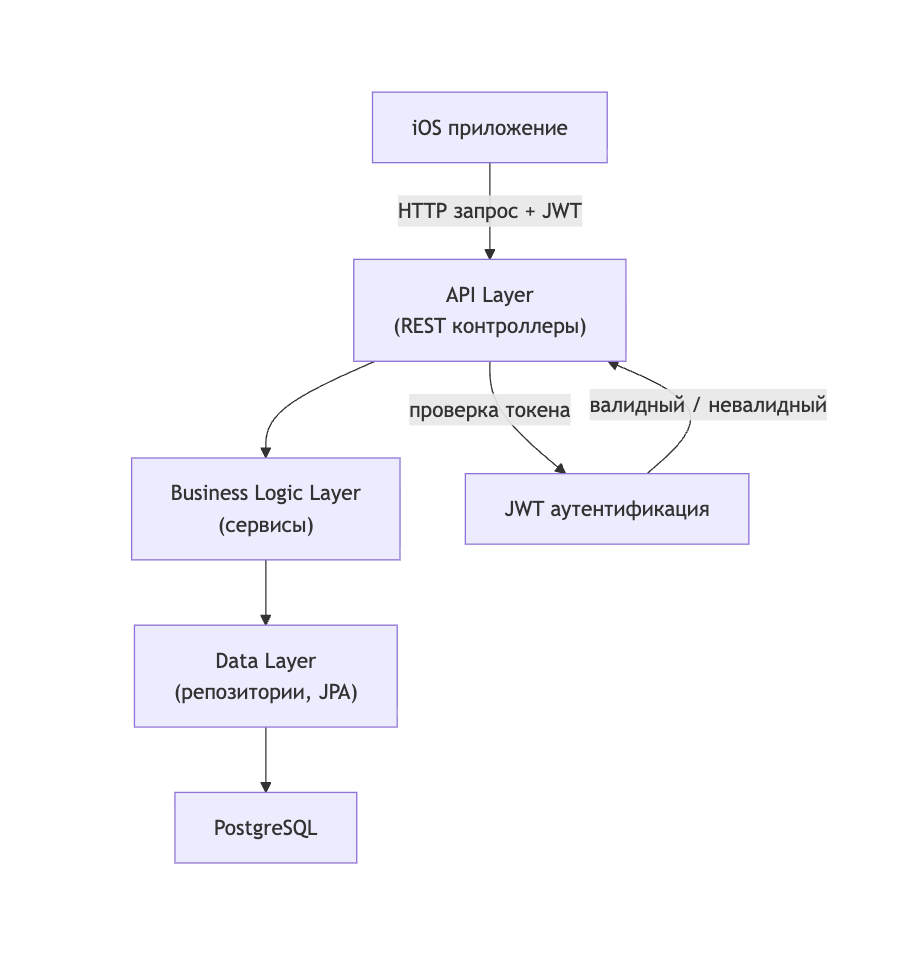
\includegraphics[width=0.85\linewidth]{my_folder/images/image17}
	\caption{Архитектура backend}
	\label{fig:17}
\end{figure}


\section{Архитектура LLM-service}


LLM-service представляет собой отдельный микросервис, реализованный на Python, предназначенный для обработки пользовательских чат-запросов. Сервис принимает текстовый запрос, выполняет поиск релевантных фрагментов Корана и формирует ответ с использованием языковой модели.


\subsection{REST API слой}


Слой REST API реализован с использованием фреймворка FastAPI и определяет HTTP-эндпоинты, через которые основной backend-сервер взаимодействует с LLM-service. Каждый эндпоинт является точкой входа для обработки определенного типа запросов и отвечает за входные данные и передачу их в последующие компоненты системы.


\subsection{RAG слой}


RAG (Retrieval-Augmented Generation) слой отвечает за поиск релевантного контекста в базе знаний. Данный слой включает следующие компоненты:

\begin{enumerate}
	\item Embeddings - выполняет преобразование текстового запроса в векторное представление.
	\item Vector Store - хранит векторные представления фрагментов Корана.
	\item Retriever - осуществляет поиск наиболее релевантных фрагментов на основе меры сходства.
\end{enumerate}

\subsection{Слой интеграции с LLM}


Слой интеграции с языковой моделью обеспечивает взаимодействие с внешним сервисом OpenRouter. В рамках данного слоя формируется запрос, включающий пользовательский ввод и найденный контекст, после чего выполняется вызов языковой модели и получение сгенерированного ответа.


\section{Макеты интерфейсов}


\begin{figure}[H]
	\centering
	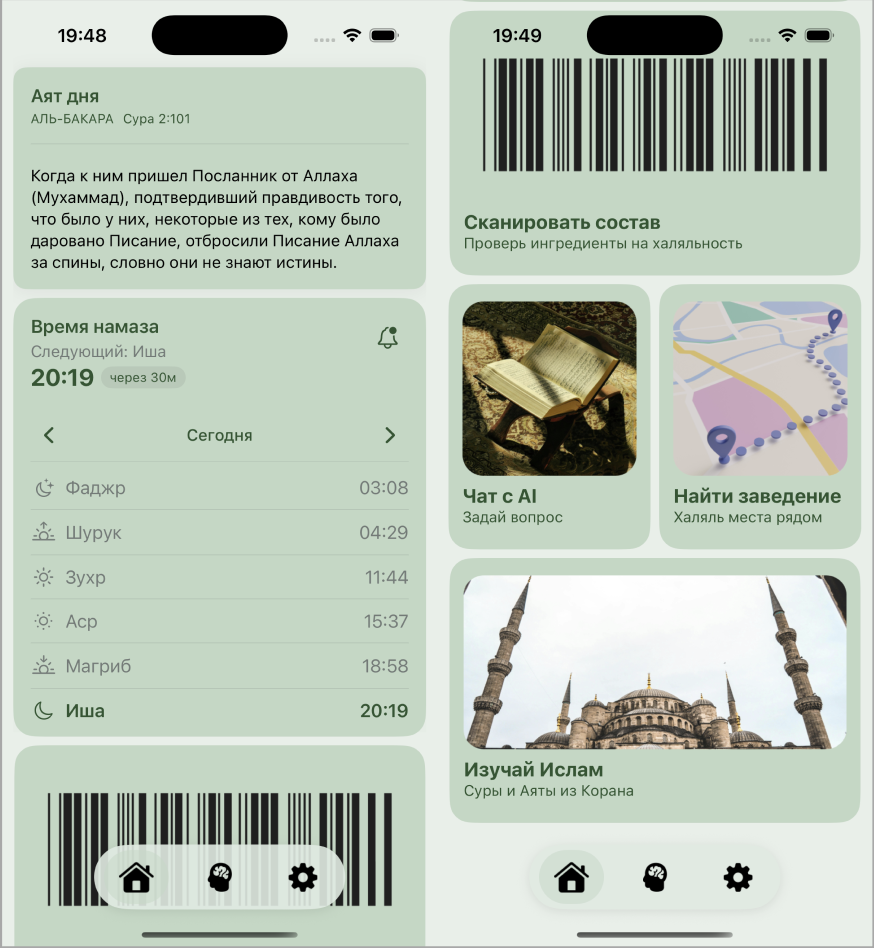
\includegraphics[width=0.85\linewidth]{my_folder/images/image18}
	\caption{Макет главного экрана}
	\label{fig:18}
\end{figure}


\begin{figure}[H]
	\centering
	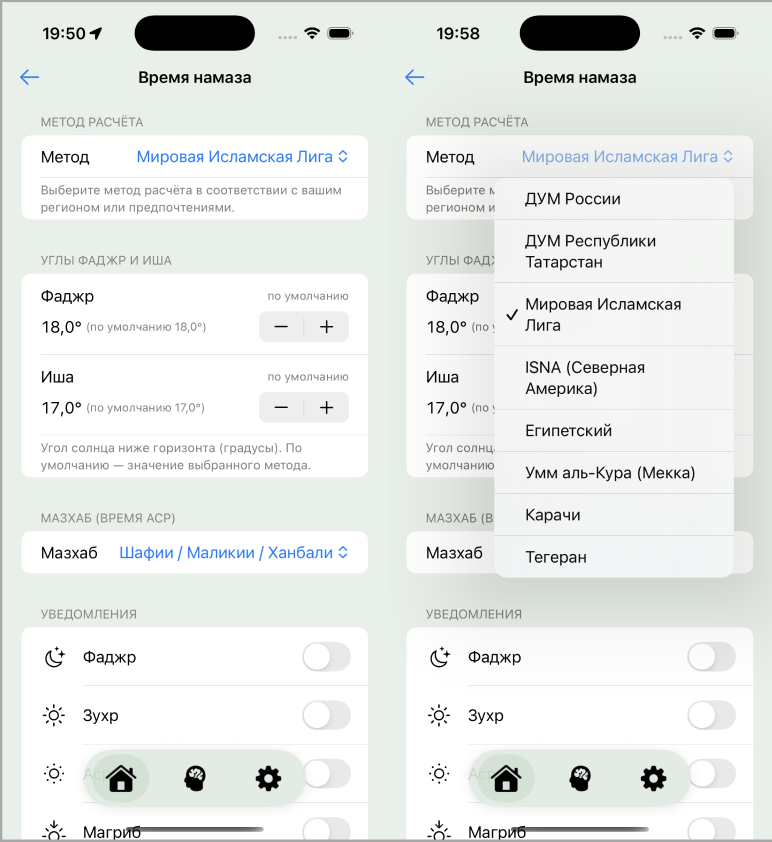
\includegraphics[width=0.85\linewidth]{my_folder/images/image19}
	\caption{Макет экрана настроек времени намаза}
	\label{fig:19}
\end{figure}


\begin{figure}[H]
	\centering
	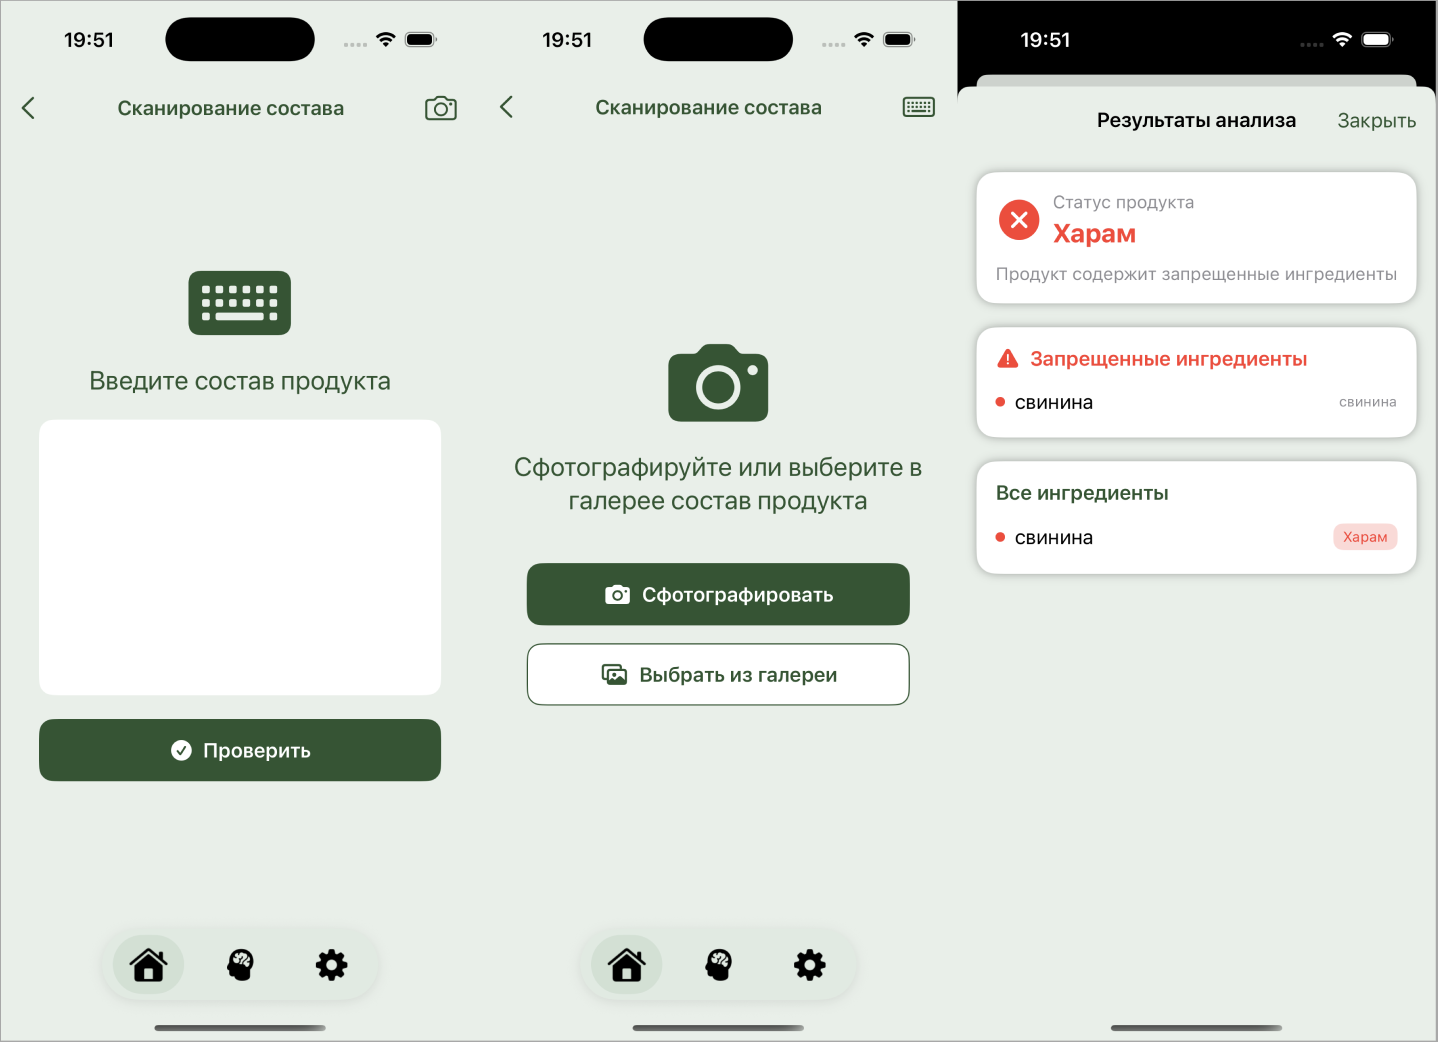
\includegraphics[width=0.85\linewidth]{my_folder/images/image20}
	\caption{Макет экрана сканирования состава продуктов}
	\label{fig:20}
\end{figure}


\begin{figure}[H]
	\centering
	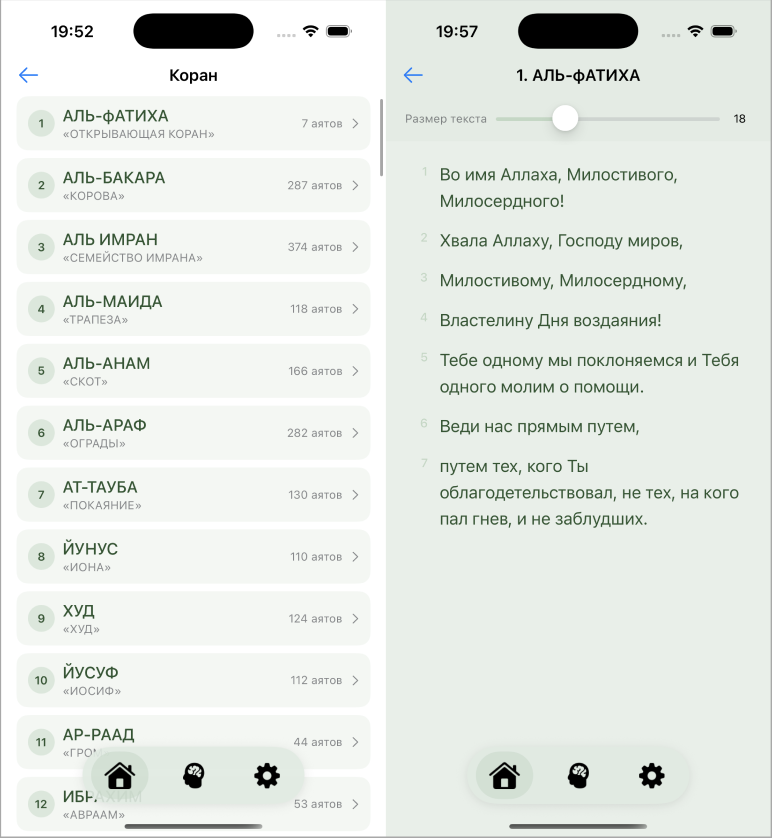
\includegraphics[width=0.85\linewidth]{my_folder/images/image21}
	\caption{Макет экрана чтения Корана}
	\label{fig:21}
\end{figure}


\begin{figure}[H]
	\centering
	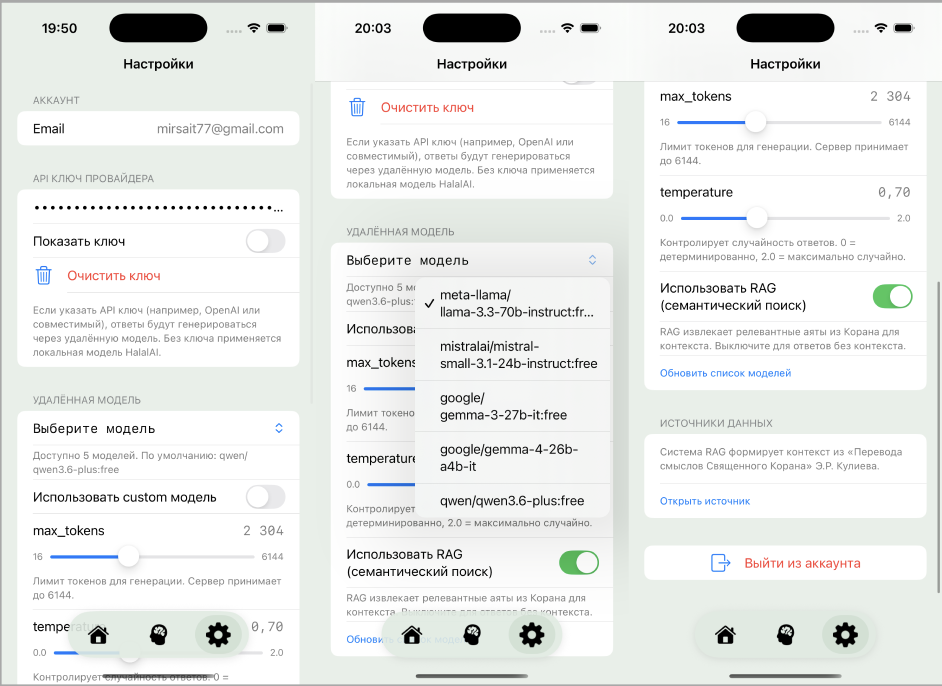
\includegraphics[width=0.85\linewidth]{my_folder/images/image22}
	\caption{Макет экрана настроек}
	\label{fig:22}
\end{figure}


\begin{figure}[H]
	\centering
	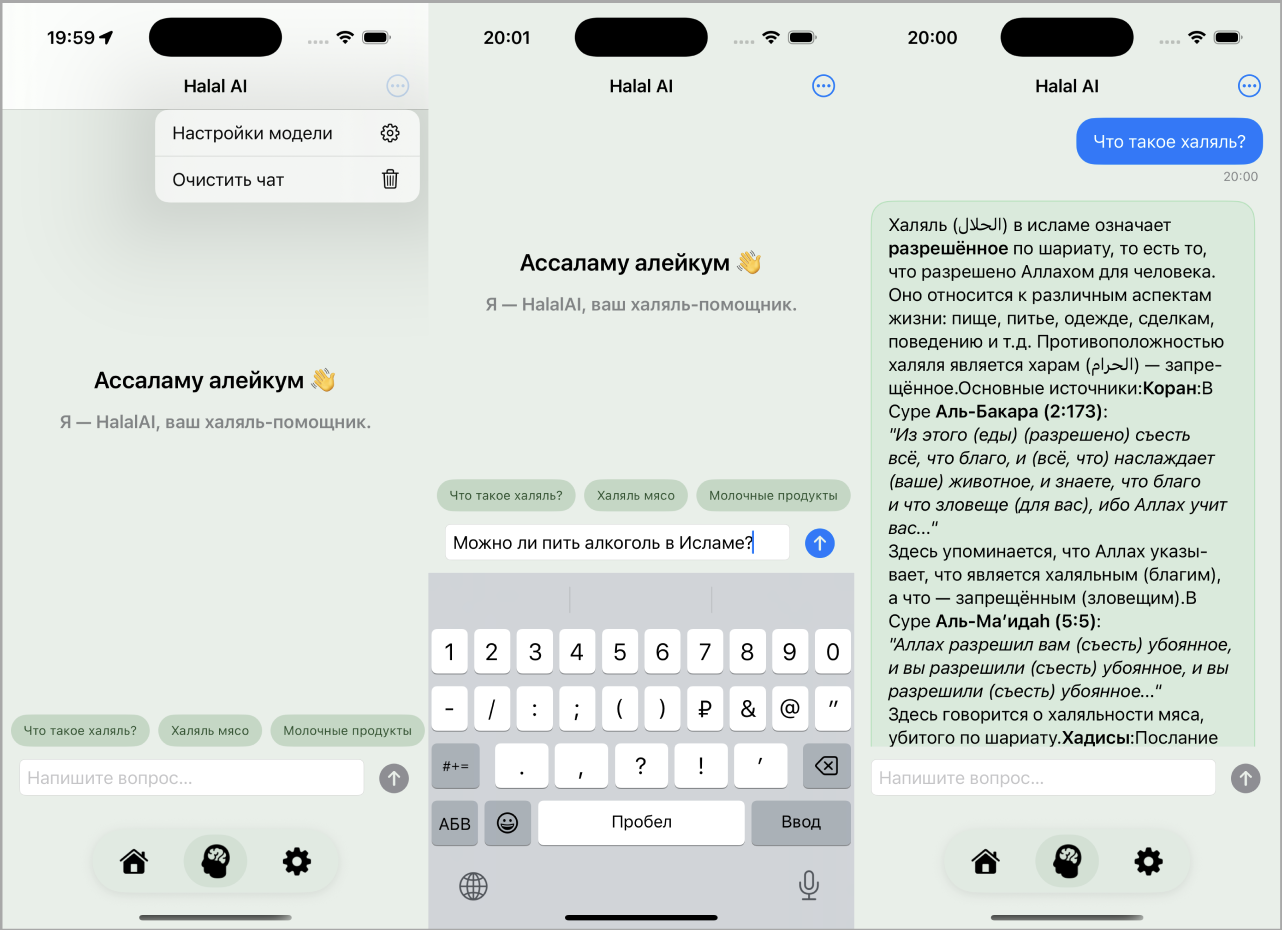
\includegraphics[width=0.85\linewidth]{my_folder/images/image23}
	\caption{Макет экрана с AI-чатом}
	\label{fig:23}
\end{figure}


\begin{figure}[H]
	\centering
	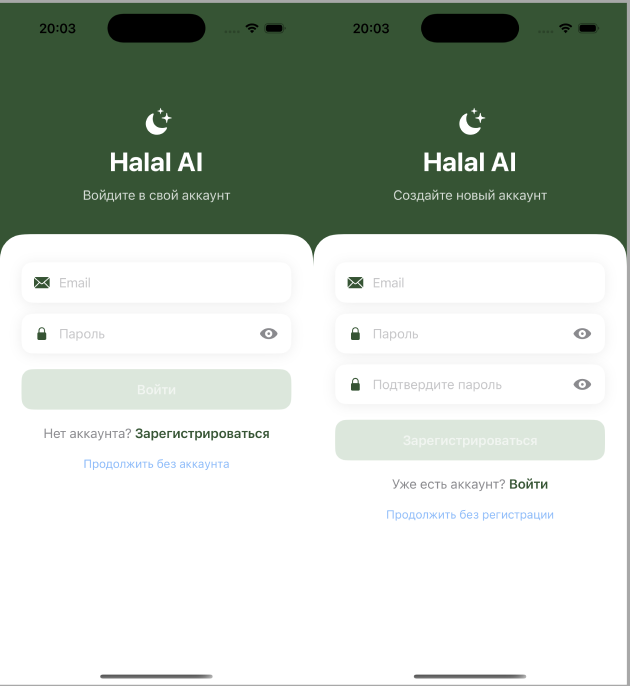
\includegraphics[width=0.85\linewidth]{my_folder/images/image24}
	\caption{Макет экранов авторизации и регистрации}
	\label{fig:24}
\end{figure}

\clearpage
